\documentclass[letterpaper,12pt,svgnames]{article}
\usepackage{CormorantGaramond}
\usepackage[T1]{fontenc}
\usepackage[english]{babel}
\usepackage[utf8]{inputenc}
\usepackage[svgnames]{xcolor}
\usepackage{fancyhdr}
\usepackage{amsmath}
\usepackage{amsfonts}
\usepackage{amssymb}
\usepackage{amsthm}
\usepackage{thmtools}
\usepackage{lipsum}
\usepackage{geometry}
\usepackage{mathtools}
\usepackage{bold-extra}
\usepackage{mathrsfs}
\usepackage{tikz}
\usepackage{tikz-cd}
\usepackage[makeroom]{cancel}
\usepackage{hanging}
\usepackage{stmaryrd}
\usepackage{enumerate}
\usepackage{soul}
\usepackage{titlesec}
\usepackage{parskip}
\usepackage{graphicx}
\usepackage{mathdots}
\usepackage{xpatch}
\usepackage{chngcntr}
\usepackage{apptools}
\usepackage[shortlabels]{enumitem}



\setenumerate[0]{label=(\alph*)}


\DeclareSymbolFont{extraup}{U}{zavm}{m}{n}
\DeclareMathSymbol{\varheart}{\mathalpha}{extraup}{86}
\DeclareMathSymbol{\vardiamond}{\mathalpha}{extraup}{87}


\makeatletter
\newcounter{savesection}
\newcounter{apdxsection}
\renewcommand\appendix{\par
  \setcounter{savesection}{\value{section}}%
  \setcounter{section}{\value{apdxsection}}%
  \setcounter{subsection}{0}%
  \gdef\thesection{\@Alph\c@section}}
\newcommand\unappendix{\par
  \setcounter{apdxsection}{\value{section}}%
  \setcounter{section}{\value{savesection}}%
  \setcounter{subsection}{0}%
  \gdef\thesection{\@arabic\c@section}}
\makeatother


% For note taking
\newcommand{\df}[1]{\textbf{\textit{#1}}}
\DeclareRobustCommand{\hlb}[1]{{\sethlcolor{DeepSkyBlue}\hl{#1}}}
\DeclareRobustCommand{\hlg}[1]{{\sethlcolor{Lime}\hl{#1}}}
\DeclareRobustCommand{\hlo}[1]{{\sethlcolor{Orange}\hl{#1}}}


\geometry{a4paper,total={168mm,248mm},left=21mm,top=22mm}

%theorems, etc.
\newtheoremstyle{mystyle}%                % Name
  {1em}%                                     % Space above
  {}%                                     % Space below
  {}%                             % Body font
  {}%                                     % Indent amount
  {\bfseries}%                            % Theorem head font
  {.}%                                    % Punctuation after theorem head
  { }%                                    % Space after theorem head, ' ', or \newline
  {}%                                     % Theorem head spec (can be left empty, meaning `normal')

\theoremstyle{mystyle}

\makeatletter
  \xpatchcmd{\@thm}{\fontseries\mddefault\upshape}{}{}{} % same font as thm-header
\makeatother


\newtheorem{thm}{Theorem}[section]
\newtheorem{lem}[thm]{Lemma}
\newtheorem{prop}[thm]{Proposition}
\newtheorem{cor}[thm]{Corollary}
\newtheorem{conj}[thm]{Conjecture}
\newtheorem{ex}[thm]{Example}


\newcommand{\dfn}{\vs\textbf{Definition. }}
\newcommand{\crly}{\vs\textbf{Corollary. }}
% \newcommand{\prp}{\vs\textbf{Proposition. }}
\newcommand{\nb}{\vs\textbf{Note: }}


\AtAppendix{\counterwithin{thm}{section}}



\usepackage[colorlinks]{hyperref}
\usepackage[nameinlink,capitalize]{cleveref}

\setlength\parindent{0pt}


%========= Spacing and format
\newcommand{\cen}{\centerline}
\newcommand{\hang}{\hangindent=0.8cm}
\newcommand{\nhang}{\hangindent=0cm}
\newcommand{\nf}{\normalfont}
\newcommand{\fl}{\noindent}
\newcommand{\vs}{\vspace{0.7em}}
\newcommand{\nl}{\textcolor{white}{nothing}}



%========= Common Math commands
\newcommand{\nin}{\not\in}
\newcommand{\ra}{\rightarrow}
\newcommand{\Ra}{\Rightarrow}
\newcommand{\La}{\Leftarrow}
\newcommand{\oa}{\overrightarrow}
\newcommand{\lbb}{\llbracket}
\newcommand{\rbb}{\rrbracket}
\newcommand{\p}{^\prime}
\newcommand{\wh}{\widehat}
\newcommand{\os}{\overset}
\newcommand{\us}{\underset}
\newcommand{\ol}{\overline}
\newcommand{\td}{\widetilde}
\newcommand{\seq}{\subseteq}
\newcommand{\lp}{\left(}
\newcommand{\rp}{\right)}
\newcommand{\lb}{\left[}
\newcommand{\rb}{\right]}
\newcommand{\im}{\text{im}}
\newcommand{\inv}{^{-1}}
\newcommand{\supp}{\text{supp}}
\newcommand{\x}{\times}
\newcommand{\Id}{\text{Id}}
\newcommand{\into}{\hookrightarrow}


%==== Greek Letter Shorthand
\newcommand{\al}{\alpha}
\newcommand{\ga}{\gamma}
\newcommand{\de}{\delta}
\newcommand{\Ga}{\Gamma}
\newcommand{\be}{\beta}
\newcommand{\Lm}{\Lambda}
\newcommand{\lm}{\lambda}
\newcommand{\Sig}{\Sigma}
\newcommand{\sig}{\sigma}
\newcommand{\Tht}{\Theta}
\newcommand{\tht}{\theta}
\newcommand{\vphi}{\varphi}
\newcommand{\vep}{\varepsilon}



%========= Linear Algebra
\newcommand{\bpm}{\begin{pmatrix}}
\newcommand{\epm}{\end{pmatrix}}
\newcommand{\bbm}{\begin{bmatrix}}
\newcommand{\ebm}{\end{bmatrix}}
\newcommand{\hh}{\hspace{2em}}
\newcommand{\vect}{\overset{\rightharpoonup}}
\newcommand{\spn}{\text{span}}


%========= Algebra notation
\newcommand{\Aut}{\text{Aut}}
\newcommand{\Inn}{\text{Inn}}
\newcommand{\Tor}{\text{Tor}}
\newcommand{\Hom}{\text{Hom}}
\newcommand{\End}{\text{End}}
\newcommand{\Gal}{\text{Gal}}
\newcommand{\Fix}{\text{Fix}}


%========= Analysis notation
\newcommand{\llp}{\left\|}
\newcommand{\rrp}{\right\|}
\newcommand{\Lin}{L^\infty}
\newcommand{\ip}[2]{\langle #1,#2\rangle} %inner product



%========= Topology notation
\newcommand{\wt}{\widetilde}
\newcommand{\es}{\varnothing}


%========= Diff. Geo Shorthand
\newcommand{\BSS}{\mathbb{S}^1}
\newcommand{\BSN}{\mathbb{S}^n}
\newcommand{\CP}{\mathbb{CP}}
\newcommand{\RP}{\mathbb{RP}}
\newcommand{\RPn}{\mathbb{RP}^n}
\newcommand{\Rn}{\mathbb{R}^n}
\newcommand{\Rm}{\mathbb{R}^m}
\newcommand{\Hn}{\mathbb{H}^n}
\newcommand{\Rk}{\mathbb{R}^k}
\newcommand{\Cin}{C^\infty}
\newcommand{\ev}[2]{\left. #1\right|_{#2}}
\newcommand{\bd}{\partial}

\newcommand{\px}{\widehat{x}}
\newcommand{\hook}{\,{\rule[0in]{2mm}{0.25mm}\rule{0.25mm}{2mm}} \, }
\newcommand{\Int}{\text{Int}}
\newcommand{\rank}{\text{rank}}
\newcommand{\Lie}{\text{Lie}}

\newcommand{\pdd}[1]{\frac{\partial}{\partial #1}}
\newcommand{\pd}[2]{\frac{\partial{#1}}{\partial{#2}}}





\titleformat{\section}[hang]{\centering\large\bfseries}{\thesection.}{1em}{}
\titleformat{\subsection}[runin]{\large\itshape}{- }{0em}{}[ -]

\fancyhf{} %these three lines put the page number at the bottom right
\rfoot{\thepage}
\renewcommand{\headrulewidth}{0pt}



\pagestyle{fancy}

\renewcommand{\qedsymbol}{$\clubsuit$}




























%========= Math letters
\newcommand{\A}{\mathbb{A}}
\newcommand{\B}{\mathbb{B}}
\newcommand{\C}{\mathbb{C}}
\newcommand{\D}{\mathbb{D}}
\newcommand{\E}{\mathbb{E}}
\newcommand{\F}{\mathbb{F}}
\newcommand{\G}{\mathbb{G}}
\newcommand{\BH}{\mathbb{H}}
\newcommand{\I}{\mathbb{I}}
\newcommand{\J}{\mathbb{J}}
\newcommand{\K}{\mathbb{K}}
\newcommand{\BL}{\mathbb{L}}
\newcommand{\BM}{\mathbb{M}}
\newcommand{\N}{\mathbb{N}}
\newcommand{\BO}{\mathbb{O}}
\newcommand{\BP}{\mathbb{P}}
\newcommand{\Q}{\mathbb{Q}}
\newcommand{\R}{\mathbb{R}}
\newcommand{\BS}{\mathbb{S}}
\newcommand{\T}{\mathbb{T}}
\newcommand{\U}{\mathbb{U}}
\newcommand{\V}{\mathbb{V}}
\newcommand{\W}{\mathbb{W}}
\newcommand{\X}{\mathbb{X}}
\newcommand{\Y}{\mathbb{Y}}
\newcommand{\Z}{\mathbb{Z}}


\newcommand{\CA}{\mathcal{A}}
\newcommand{\BB}{\mathcal{B}}
\newcommand{\CC}{\mathcal{C}}
\newcommand{\DD}{\mathcal{D}}
\newcommand{\EE}{\mathcal{E}}
\newcommand{\FF}{\mathcal{F}}
\newcommand{\GG}{\mathcal{G}}
\newcommand{\HH}{\mathcal{H}}
\newcommand{\II}{\mathcal{I}}
\newcommand{\JJ}{\mathcal{J}}
\newcommand{\KK}{\mathcal{K}}
\newcommand{\LL}{\mathcal{L}}
\newcommand{\MM}{\mathcal{M}}
\newcommand{\NN}{\mathcal{N}}
\newcommand{\OO}{\mathcal{O}}
\newcommand{\PP}{\mathcal{P}}
\newcommand{\QQ}{\mathcal{Q}}
\newcommand{\RR}{\mathcal{R}}
\newcommand{\CS}{\mathcal{S}}
\newcommand{\TT}{\mathcal{T}}
\newcommand{\UU}{\mathcal{U}}
\newcommand{\VV}{\mathcal{V}}
\newcommand{\WW}{\mathcal{W}}
\newcommand{\XX}{\mathcal{X}}
\newcommand{\YY}{\mathcal{Y}}
\newcommand{\ZZ}{\mathcal{Z}}

\newcommand{\fA}{\mathscr{A}}
\newcommand{\fB}{\mathscr{B}}
\newcommand{\fC}{\mathscr{C}}
\newcommand{\fD}{\mathscr{D}}
\newcommand{\fE}{\mathscr{E}}
\newcommand{\fF}{\mathscr{F}}
\newcommand{\fG}{\mathscr{G}}
\newcommand{\fH}{\mathscr{H}}
\newcommand{\fI}{\mathscr{I}}
\newcommand{\fJ}{\mathscr{J}}
\newcommand{\fK}{\mathscr{K}}
\newcommand{\fL}{\mathscr{L}}
\newcommand{\fM}{\mathscr{M}}
\newcommand{\fN}{\mathscr{N}}
\newcommand{\fO}{\mathscr{O}}
\newcommand{\fP}{\mathscr{P}}
\newcommand{\fQ}{\mathscr{Q}}
\newcommand{\fR}{\mathscr{R}}
\newcommand{\fS}{\mathscr{S}}
\newcommand{\fT}{\mathscr{T}}
\newcommand{\fU}{\mathscr{U}}
\newcommand{\fV}{\mathscr{V}}
\newcommand{\fW}{\mathscr{W}}
\newcommand{\fX}{\mathscr{X}}
\newcommand{\fY}{\mathscr{Y}}
\newcommand{\fZ}{\mathscr{Z}}


\newcommand{\fkA}{\mathfrak{A}}
\newcommand{\fkB}{\mathfrak{B}}
\newcommand{\fkC}{\mathfrak{C}}
\newcommand{\fkD}{\mathfrak{D}}
\newcommand{\fkE}{\mathfrak{E}}
\newcommand{\fkF}{\mathfrak{F}}
\newcommand{\fkG}{\mathfrak{G}}
\newcommand{\fkH}{\mathfrak{H}}
\newcommand{\fkI}{\mathfrak{I}}
\newcommand{\fkJ}{\mathfrak{J}}
\newcommand{\fkK}{\mathfrak{K}}
\newcommand{\fkL}{\mathfrak{L}}
\newcommand{\fkM}{\mathfrak{M}}
\newcommand{\fkN}{\mathfrak{N}}
\newcommand{\fkO}{\mathfrak{O}}
\newcommand{\fkP}{\mathfrak{P}}
\newcommand{\fkQ}{\mathfrak{Q}}
\newcommand{\fkR}{\mathfrak{R}}
\newcommand{\fkS}{\mathfrak{S}}
\newcommand{\fkT}{\mathfrak{T}}
\newcommand{\fkU}{\mathfrak{U}}
\newcommand{\fkV}{\mathfrak{V}}
\newcommand{\fkW}{\mathfrak{W}}
\newcommand{\fkX}{\mathfrak{X}}
\newcommand{\fkY}{\mathfrak{Y}}
\newcommand{\fkZ}{\mathfrak{Z}}

\newcommand{\fka}{\mathfrak{a}}
\newcommand{\fkb}{\mathfrak{b}}
\newcommand{\fkc}{\mathfrak{c}}
\newcommand{\fkd}{\mathfrak{d}}
\newcommand{\fke}{\mathfrak{e}}
\newcommand{\fkf}{\mathfrak{f}}
\newcommand{\fkg}{\mathfrak{g}}
\newcommand{\fkh}{\mathfrak{h}}
\newcommand{\fki}{\mathfrak{i}}
\newcommand{\fkj}{\mathfrak{j}}
\newcommand{\fkk}{\mathfrak{k}}
\newcommand{\fkl}{\mathfrak{l}}
\newcommand{\fkm}{\mathfrak{m}}
\newcommand{\fkn}{\mathfrak{n}}
\newcommand{\fko}{\mathfrak{o}}
\newcommand{\fkp}{\mathfrak{p}}
\newcommand{\fkq}{\mathfrak{q}}
\newcommand{\fkr}{\mathfrak{r}}
\newcommand{\fks}{\mathfrak{s}}
\newcommand{\fkt}{\mathfrak{t}}
\newcommand{\fku}{\mathfrak{u}}
\newcommand{\fkv}{\mathfrak{v}}
\newcommand{\fkw}{\mathfrak{w}}
\newcommand{\fkx}{\mathfrak{x}}
\newcommand{\fky}{\mathfrak{y}}
\newcommand{\fkz}{\mathfrak{z}}


\newcommand{\ba}{\textbf{a}}
\newcommand{\bb}{\textbf{b}}
\newcommand{\bc}{\textbf{c}}
\newcommand{\bdd}{\textbf{d}}
\newcommand{\bde}{\textbf{e}}
\newcommand{\bdf}{\textbf{f}}
\newcommand{\bg}{\textbf{g}}
\newcommand{\bh}{\textbf{h}}
\newcommand{\bi}{\textbf{i}}
\newcommand{\bj}{\textbf{j}}
\newcommand{\bk}{\textbf{k}}
\newcommand{\bl}{\textbf{l}}
\newcommand{\bm}{\textbf{m}}
\newcommand{\bn}{\textbf{n}}
\newcommand{\bo}{\textbf{o}}
\newcommand{\bp}{\textbf{p}}
\newcommand{\bq}{\textbf{q}}
\newcommand{\br}{\textbf{r}}
\newcommand{\bs}{\textbf{s}}
\newcommand{\bt}{\textbf{t}}
\newcommand{\bu}{\textbf{u}}
\newcommand{\bv}{\textbf{v}}
\newcommand{\bw}{\textbf{w}}
\newcommand{\bx}{\textbf{x}}
\newcommand{\by}{\textbf{y}}
\newcommand{\bz}{\textbf{z}}

\usepackage{color}

\newcommand{\fkgl}{\mathfrak{gl}}
\newcommand{\op}{^{(p)}}
\newcommand{\dfng}{\vs\textbf{\hlg{Definition.}} }
\newcommand{\bgw}{\Lambda}


\title{Crazy Geometry Project}

\newcommand{\wowob}{with or without boundary}


\begin{document}
\begin{center}
\textbf{\Large Differential Geometry Preliminary Exam Notes}
\end{center}

This is a list of most of the definitions, theorems, and propositions contained within \textit{Introduction to Smooth Manifolds} by John M. Lee as well as some extra useful ones. All the numbered theorems within this set of notes should correspond with the actual numbering of the theorems within the book. 

Also, in these notes \hl{we will conform to the Einstein summation convention.}

Important things that really, really need to be remembered will be \hlb{highlighted in blue.} Things to keep in mind are \hl{highlighted in yellow}, important definitions are \hlg{highlighted in green}, and good examples are \hlo{highlighted in orange.}

\tableofcontents
\newpage

\appendix
\setcounter{section}{2}
\section{Appendix C Review of Calculus}
\setcounter{thm}{0}

\dfn Let $V, W$ be finite-dimensional vector spaces. If $U\subset V$ is an open subset and $a\in U$, a map $F:U\ra W$ is said to be \textbf{\textit{differentiable at a}} if there exists a linear map $L:V\ra W$ such that
\[\lim_{v\ra 0} \frac{|F(a + v) - F(a) - Lv|}{|v|} = 0.\]
If $F$ is differentiable at $a$, the linear map $L$ satisfying this condition is denoted $DF(a)$ and is called the \textbf{\textit{total derivative of $\boldsymbol F$ at $\boldsymbol a$}}. This condition may also be written as 
\[F(a + v) = F(a) + DF(a)v + R(v)\]
where $R(v)$ satisfies $|R(v)|/|v| \ra 0$ as $v\ra 0$.

\setcounter{thm}{2}

\begin{prop}[The Chain Rule for Total Derivatives]
Suppose $V, W, X$ are finite-dimensional vector spaces, $U\subset V$ ad $\td U \subset W$ are open subsets, and $F:U\ra \td U$ and $G:\td U \ra X$ are maps. If $F$ is differentiable at $a\in U$ and $G$ is differentiable at $F(a)\in \td U$, then $G\circ F$ is differentiable at $a$, and 
\[D(G\circ F)(a) = DG(F(a)) \circ DF(a).\]
\end{prop}


\dfn Suppose $U\subset \R^n$ is open and $f:U\ra \R$ is a real-valued function. For any $a = (a^1, \ldots, a^n)\in U$ and any $j\in \{1,\ldots, n\}$, the \textbf{$\boldsymbol{j^{th}}$ partial derivative of $\boldsymbol f$ at $\boldsymbol a$} is defined to be
\[\pd{f}{x^j}(a) = \lim_{h\ra 0}\frac{f(a + he_j) = f(a)}{h},\]
where $e_j$ is the $j^{th}$ elementary basis vector for $\R^n$.


\dfn For vector-valued functions $F:U\ra \R^m$, we can write the coordinates of $F(x)$ as $F(x) = (F^1(x),\ldots, F^m(x))$. These $m$ functions are called the \textbf{\textit{component functions of $\boldsymbol{F}$}}. The matrix of partial derivatives of the component functions given by 
\[J = \lp\frac{\partial F^i}{\partial x^j}\rp\]
is called the \textbf{\textit{Jacobian matrix of $\boldsymbol{F}$}}.


\dfn If $F:U\ra \R^m$ is a function for which the partial derivative exists at each point in $U$ and the functions $\partial F^i/\partial x^j:U \ra \R$ are all continuous, then $F$ is said to be of \textbf{\textit{class $\boldsymbol{C^1}$}} or \textbf{\textit{continuously differentiable}}. The \textbf{\textit{second-order partial derivatives}} can be obtained by
\[\frac{\partial^2 F^i}{\partial x^k \partial x^j} = \frac{\partial}{\partial x^k}\lp \frac{\partial F^i}{\partial x^j}\rp\]
and continuing in this way we can obtain the \textbf{\textit{partial derivatives of $\boldsymbol{F}$ of order $\boldsymbol{k}$}}. A function is function $F:U\ra \R^m$ is said to be of \textbf{\textit{class $\boldsymbol{C^k}$}} if all the partial derivatives of $F$ of order less than or equal to $k$ exist and are continuous functions on $U$. A function is called \textbf{\textit{smooth}} if it is of class $\Cin$.



\dfn If $U$ and $V$ are open subsets of Euclidean spaces, a function $F:U\ra V$ is called a \textit{\textbf{diffeomorphism}} if it is smooth and bijective and its inverse function is also smooth.

\setcounter{thm}{3}

\begin{prop}
Suppose $U\seq \R^n$ and $V\seq R^m$ are open subsets and $F:U\ra V$ is a diffeomorphism. Then $m = n$, and for each $a\in U$, the total derivative $DF(a)$ is invertible, with $DF(a)\inv = D(F\inv)(F(a))$.
\end{prop} 

\setcounter{thm}{5}

\begin{prop}[Equality of Mixed Partial Derivatives]
If $U$ is an open subset of $\Rn$ and $F:U\ra \Rm$ is a function of class $C^2$, then the mixed second-order partial derivatives of $F$ do not depend on the order of differentiation:
\[\frac{\partial^2F^i}{\partial x^j\partial x^k} = \frac{\partial^2F^i}{\partial x^k\partial x^j}.\]
\end{prop}



\crly If $F:U\ra \Rm$ is smooth, then the mixed partial derivatives of $F$ of any order are independent of the order of differentiation.

\setcounter{thm}{7}

\begin{prop}
Let $U\seq \Rn$ be open, and suppose $F:U \ra \Rm$ is differentiable at $a\in U$. Then all of the partial derivatives of $F$ at $a$ exist, and $DF(a)$ is the linear map whose matrix is the Jacobian of $F$ at $a$:
\[DF(a) = \lp\pd{F^j}{x^i}(a)\rp.\]
\end{prop}


\setcounter{thm}{9}

\begin{prop}
 Let $U\seq \Rn$ be open. If $F:U\ra \Rm$ is of class $C^1$, then it is differentiable at each point of $U$.
\end{prop}

\begin{cor}[The Chain Rule for Partial Derivatives]
Let $U\seq \Rn$ and $\td U\seq \Rm$ be open subsets, and let $x = (x^1, \ldots, x^n)$ denote the standard coordinates on $U$, and $y = (y^1, \ldots, y^m)$ those on $\td U$.
\begin{enumerate}
    \item A composition of $C^1$ function $F:U\ra \td U$ and $G:\td U\ra \R^p$ is again of class $C^1$, with partial derivatives given by 
    \[\pd{(G^i\circ F)}{x^j}(x) = \sum_{k = 1}^m\pd{G^i}{y^k}(F(x))\pd{F^k}{x^j}(x).\]
    \item If $F$ and $G$ are smooth, then $G\circ F$ is smooth.
\end{enumerate}
\end{cor}


\dfn Suppose $f:U\ra \R$ is a smooth real-valued function on an open subset $U\seq \Rn$, and $a\in U$. For each vector $\bv\in \Rn$, we define the \textbf{\textit{directional derivative of $\boldsymbol{f}$ in the direction of v at $\boldsymbol{a}$}} to be the number
\[D_\bv f(a) = \ev{\frac{d}{dt}}{t = 0}\pd{f}{x^i}(a) = Df(a)\bv\]


\setcounter{thm}{33}
\begin{thm}[\hlb{Inverse Function Theorem}]\label{C_inv_fct}
Suppose $U$ and $V$ are open subsets of $\Rn$, and $F:U\ra V$ is a smooth function. If $DF(a)$ is invertible at some point $a\in U$
\end{thm}

\dfn Let $X$ be a metric space. A map $G:X\ra X$ is said to be a \textbf{\textit{contraction}} if there is a constant $\lm\in (0,1)$ such that $d(G(x), G(y)) \leq \lm\,d(x,y)$ for all $x,y\in X$. A \textbf{\textit{fixed point}} of a map $G:X\ra X$ is a point $x\in X$ such that $G(x) = x$.

\begin{lem}[Contraction Lemma]
Let $X$ be a nonempty complete metric space. Every contraction $G:X\ra X$ has a unique fixed point.
\end{lem}

\begin{cor}
uppose $U\seq\Rn$ is an open subset, and $F:U\ra \Rn$ is a smooth function whose Jacobian determinant is nonzero at every point in $U$.
\begin{enumerate}
    \item $F$ is an open map.
    \item If $F$ is injective, then $F:U\ra F(U)$ is a diffeomorphism.
\end{enumerate}
\end{cor}

\begin{thm}[\hlb{Implicit Function Theorem}]
Let  $U\seq \Rn\x\Rk$ be an open subset, and let $(x,y) = (x^1,\ldots,x^n,y^1,\ldots,y^k)$ denote the standard coordinates on $U$. Suppose $\Phi:U\ra \Rk$ is a smooth function, $(a,b)\in U$, and $c\in \Phi(a,b)$. If the $k\x k$ matrix
\[\lp\pd{\Phi^i}{y^j}(a,b)\rp\]
is nonsingular, then there exist neighborhoods $v_0\seq \Rn$ of $a$ and $W_0\seq \Rk$ of $b$ and a smooth function $F:V_0\ra \W_0$ such that $\Phi\inv(c)\cap (V_0\x W_0)$ is the graph of $F$, that is, $\Phi(x,y) = c$ for $(x,y)\in V_0\x W_0$ if and only if $y = F(x)$.
\end{thm}


\nb This theorem is very, very useful for any proofs involving maps between smooth charts that have sufficiently "nice" local coordinate expressions. You 100\% need this theorem for the prelim exam.

































































\newpage
\unappendix
\section{Smooth Manifolds}


When dealing with smooth manifolds, the idea that you want to keep in mind is that, locally, they all are supposed to look like a section of $\Rn$. As such, a good chunk of Differential Geometry deals with the ways in which we may extend our understanding of $\Rn$ to generalized differentiable manifolds. There is actually a very nice theorem (called the Whitney Embedding Theorem which will be discussed in a later section) that tells us that all smooth manifolds of dimension $n$ can be embedded in a space of dimension $\R^{2n + 1}$. But that is a topic that will not be covered until the section on Sard's Theorem. For now, we will work on how, exactly, we define smooth manifolds, and give ourselves some tools for doing Calculus on them.


\subsection{Definition of a Smooth Manifold}
\nl

\dfn We say that a topological space $M$ is a \textbf{\textit{topological n-manifold}} if 
\begin{itemize}
    \item $M$ is a Hausdorff space.
    \item $M$ is second-countable.
    \item \hl{$M$ is locally Euclidean of dimension $n$.} That is, every point $p\in M$ has a neighborhood that is homeomorphic to $\Rn$ for a fixed $n$. This means that for each $p\in M$ we can find
    \begin{itemize}
        \item an open neighborhood $U\seq M$ around $p$,
        \item an open neighborhood $\wh U\seq \Rn$, and 
        \item a homeomorphism $\vphi: U\ra \wh U$.
    \end{itemize}
\end{itemize}


\setcounter{thm}{1}

\begin{thm}[Topological Invariance of Dimension]
A non-empty topological $n$-manifold cannot be homeomorphic to a topological $m$-manifold unless $m = n$.
\end{thm}

\dfn Let $M$ be a topological $n$-manifold. A \textbf{\textit{coordinate chart}} on $M$ is an ordered pair $(U, \vphi)$, where $U$ is an open subset of $M$ (called the \textbf{\textit{coordinate domain}}) and $\vphi:U\ra \wh U$ is a homeomorphism from $U$ to an open subset $\wh U = \vphi(U) \seq \Rn$. If $\vphi(p) = 0$ for $p\in U$, then we say that the chart is \textbf{\textit{centered at p}}.

\begin{center}
    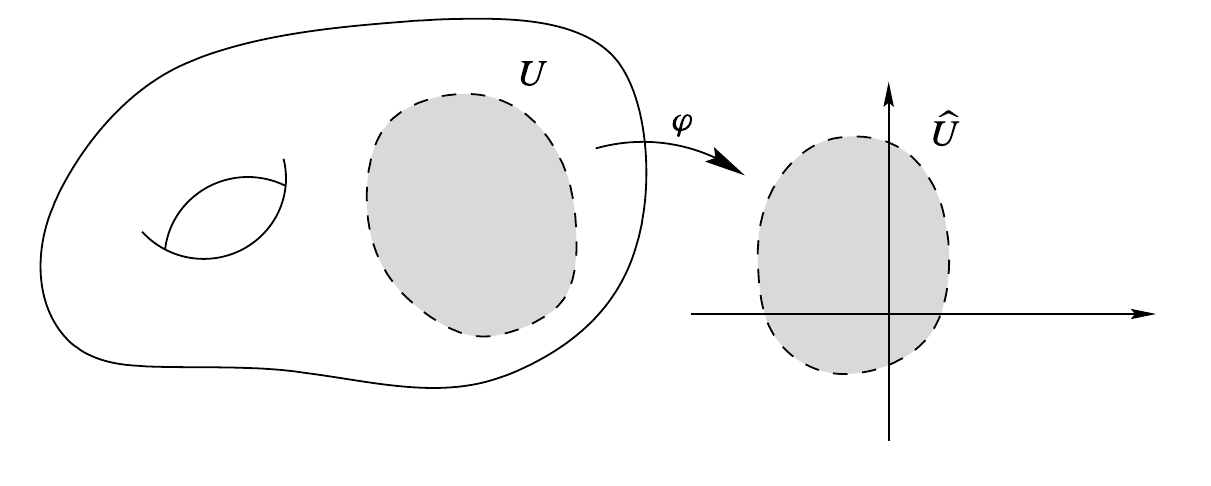
\includegraphics[scale = 0.4]{chapter01/c1f2.png}
\end{center}

\setcounter{thm}{10}

\begin{prop}
Let $M$ be a topological manifold. 
\begin{enumerate}
    \item $M$ is locally path connected.
    \item $M$ is connected if and only if it is path-connected.
    \item \hl{The components of $M$ are the same as its path components.}
    \item $M$ has countably many components, each of which is an open subset of $M$ and a connected topological manifold.
\end{enumerate}
\end{prop}

\begin{prop}
Every topological manifold is locally compact.
\end{prop}

\dfn Let $M$ be a topological space. A collection $\XX$ of subsets of $M$ is said to be \textbf{\textit{locally finite}} if each point of $M$ has a neighborhood that intersects at most finitely many members of $\XX$. 

\dfn Given a cover $\UU$ pf $M$, another cover $\VV$ is called a \textbf{\textit{refinement of $\boldsymbol{\UU}$}} if for each $V\in \VV$ there is some $U\in \UU$ such that $V\seq U$. We say that $M$ is \textbf{\textit{paracompact}} if every open cover of $M$ admits an open, locally finite refinement.

\setcounter{thm}{14}

\begin{thm}[Manifolds are Paracompact]
Every topological manifold is paracompact. In fact, given a topological manifold $M$, an open cover $\XX$ of $M$, and any basis $\BB$ for the topology on $M$, there exists a countable, locally finite open refinement of $\XX$ consisting of elements of $\BB$.
\end{thm}

\dfn If $U$ and $V$ are open subsets of Euclidean spaces $\Rn$ and $\Rm$, respectively, a function $F:U\ra V$ is said to be \hl{\textbf{\textit{smooth}}} if each of its component functions has continuous partial derivatives of all orders. If in addition $F$ is bijective and has a smooth inverse map, it is called a \hl{\textbf{\textit{diffeomorphism}}}.

\dfn Let $M$ be a topological $n$-manifold. If $(U, \vphi)$, $(V,\psi)$ are two charts such that $U\cap V\neq \es$, the composite map $\psi\circ\vphi\inv:\phi(U\cap V) \ra \psi(U\cap V)$ is called the \textbf{\textit{transition map from $\boldsymbol{\vphi}$ to $\boldsymbol{\psi}$}}. It is a composition of homeomophsims, and is therefore itself a homeomorphism. Two charts $(U,\vphi)$ and $(V,\psi)$ are said to be \textbf{\textit{smoothly compatible}} if either $U\cap V = \es$ or the transition map $\psi\circ\vphi\inv$ is a diffeomorphism.

\begin{center}
    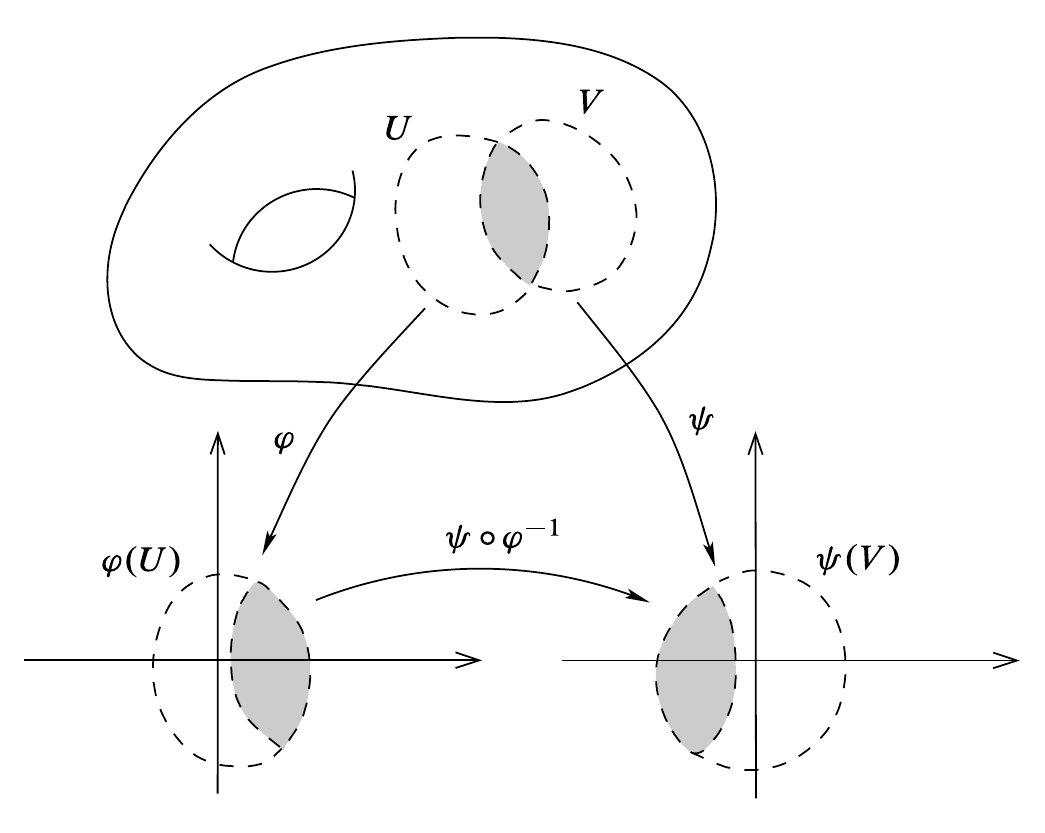
\includegraphics[scale = 0.4]{chapter01/c1f6.png}
\end{center}

\dfn An \textbf{\textit{atlas}} for a manifold $M$ is a collection of charts whose domains cover $M$. An atlas $\CA$ is called a \textbf{\textit{smooth atlas}} if any two charts in $\CA$ are smoothly compatible.

\nb Given two particular charts $(U, \vphi)$ and $(V,\psi)$, \hl{it is often easiest to show that they are smoothly compatible} by verifying that $\psi\circ\vphi\inv$ is smooth and injective with nonsingular Jacobian at each point, and appealing to Corollary C.36.

\dfn A smooth atlas $\CA$ in $M$ is \textbf{\textit{maximal}} if it is not properly contained in any larger smooth atlas. 

\dfn If $M$ is a topological manifold, a \textbf{\textit{smooth structure on M}} is a maximal smooth atlas. A \hl{\textbf{\textit{smooth manifold}}} is a pair $(M, \CA)$, where $M$ is a topological manifold and $\CA$ is a smooth structure on $M$.

\setcounter{thm}{16}

\begin{thm}Let $M$ be a topological manifold.
\begin{enumerate}
    \item Every smooth atlas $\CA$ for $M$ is contained in a unique maximal smooth atlas, called the \textbf{\textit{smooth structure determined by $\boldsymbol{\CA}$}}.
    \item Two smooth atlases for $M$ determine the same smooth structure if and only if their union is a smooth atlas.
\end{enumerate}
\end{thm}

\dfn If $M$ is a smoothm manifold, any chart $(U, \vphi)$ contained in th given maximal smooth atlas is called a \textbf{\textit{smooth chart}}, and the corresponding coordinate map $\vphi$ is called a \textbf{\textit{smooth coordinate map}}.

\subsection{Examples of Smooth Manifolds}

\setcounter{thm}{21}

\begin{ex}[Euclidean Spaces]
For each nonnegetive integer $n$, the Euclidean space $\Rn$ is a smooth $n$-manifold with the smooth structure determined by the atlas consisting of the single chart $(\Rn, \Id_\Rn)$. We call this the \textbf{\textit{standard smooth structure on $\boldsymbol{\Rn}$}} and the resulting coordinate map \textbf{\textit{standard coordinates}}. Unless we explicitly specify otherwise, we always use this smooth structure on $\Rn$. With respect to this smooth structure, the smooth coordinate charts for $\Rn$ are exactly those charts $(U,\vphi)$ such that $\vphi$ is a diffeomorphism from $U$ to another open subset $\wh U\seq \Rn$.
\end{ex}

\setcounter{thm}{24}

\begin{ex}[Spaces of Matrices]
Let $M(m\x n, \R)$ denote the set of $m\x n$ matrices with real entries. Because it is a real vector space of dimension $mn$ under matrix addition and scalar multiplication, $M(m\x n, \R)$ is a smooth $mn$-dimensional manifold. Similarly, the space $M(m\x n, \C)$ of $m\x n$ complex matrices is a vector space of dimension $2mn$ over $\R$, and thus a smooth manifold of dimension $2mn$.
\end{ex}

\begin{ex}[Open Submanifolds]
Let $U$ be any open subset of $\Rn$. Then $U$ is a topological $n$-manifold, and the single chart $(U, \Id_U)$ defines a smooth structure on $U$.

More generally, let $M$ be a smooth $n$-manifold and let $U\seq M$ be any open subset. Define an atlas on $U$ by
\[\CA_U = \{\text{smooth charts $(V, \vphi)$ for $M$ such that $V\seq U$}\}\]
Every point $p\in U$ is contained in the domain of some chart $(W, \vphi)$ for $M$; if we set $V = W\cap U$, then $(V,\vphi|_V)$ is a chart in $\CA_U$ whose domain contains $p$. It is then easy to verify that $\CA_U$ is a maximal smooth atlas for $U$, and thus any open subset of $M$ is itself a smooth $n$-manifold in a natural way. Endowed with this smooth structure, we call any open subset an \textbf{\textit{open submanifold of M}} (indeed, this will turn out to be motivation for how we define an \textit{Embedded Submanifold} later on in chapter 5).
\end{ex}

\begin{ex}[\hlo{The General Linear Group}]
The general linear group $GL(n(\R)$ is the set of $n\x n$ matrices with real entries. It is a smooth $n^2$-dimensional manifold because it is an open subset of the $n^2$-dimensional vector space $M_n(\R)$, namely the set where the (continuous) determinant function is nonzero.
\end{ex}

\setcounter{thm}{30}

\begin{ex}[Spheres]
We know that the $n$-sphere $\BSN\seq \R^{n + 1}$ is a topological $n$-manifold. We put a smooth structure on $\BSN$ as follows. For each $i = 1..n + 1$, let $(U_i^\pm. \vphi_i^\pm)$ denote the graph coordinate charts given by 
\[U_i^\pm = \{(x^1, \ldots, x^{n + 1}\in \R^{n + 1}\ :\ \pm x^i > 0\}\]
and 
\[\vphi_i^\pm (x^1,\ldots,x^{n + 1}) = (x^1,\ldots,\wh x^i,\ldots x^{n + 1}).\]
For any distinct indices $i$ and $j$, the transition map $\vphi_i^\pm\circ(\vphi^\pm)\inv$ is easily computed. In the case where $i < j$, we get 
\[\vphi_i^pm\circ(\vphi_j^\pm)\inv(u^1, \ldots, u^n) = \lp u^1,\ldots,\wh u^1,\ldots,\pm\sqrt{1 = |u|^2},\ldots,u^n\rp\]
and a similar formula holds when $i > j$. When $i = j$, $\vphi_i^+\circ(\vphi_i^-)\inv = \vphi_i^-\circ (\vphi_i^+)\inv = \Id_{\B^n}$. Thus the collection of charts $\{(\U_i^\pm, \vphi_i^\pm)\}$ is a smooth atlas, as so defines a smooth structure on $\BSN$. We call this its \textbf{\textit{standard smooth structure}}.
\end{ex}

\begin{ex}[\hlo{Level Sets}]
We can actually generalize the preceding example in the following way. Suppose $U\seq \Rn$ is an open subset and $\Phi:U\ra \R$ is a smooth function. For any $c\in \R$, the set $\Phi\inv(c)$ is called a \textbf{\textit{level set of $\boldsymbol{\Phi}$}}. Choose some $c\in \R$, let $M = \Phi\inv(c)$, and suppose it happens that the total derivative $D\Phi(a)$ is nonzero for each $a\in \Phi\inv(c)$. Because $D\Phi(a)$ is a row matrix whose entries are the partial derivatives $\lp\pd{\Phi}{x^1}(a),\ldots,\pd{\Phi}{x^n}(a)\rp$, for each $a\in M$ there is some $i$ such that $\pd{\Phi}{x^i}(a)\neq 0$. It follow from the Implicit Function Theorem, that there is a neighborhood $U_0$ of $a$ such that $M\cap U_0$ can be expressed as the graphi of an equation of the form 
\[x^i = f(x^1,\ldots,\wh x^i, \ldots, x^n),\]
for some smooth real-valued function $f$ defined on an open subset of $\R^{n - 1}$. Therefore, arguing just as in the case of the $n$-sphere, we wee that $M$ is a topological manifold of dimension $(n -1)$, and has a smooth structure such that each of the graph coordinate charts associated with a choice of $f$ as above is a smooth chart. 
\end{ex}

\begin{ex}[Projective Spaces]
The $n$-dimensional real projective space $\RPn$ is a topological $n$-manifold when given coordinate charts as in Example 1.5 of the Lee book. If we assume for convenience that $i > j$, then we can get
\[\vphi_j\circ\vphi_i\inv(u^1,\ldots,u^n) = \lp\frac{u^1}{u^j},\ldots,\frac{u^{j - 1}}{u^j},\frac{u^{j + 1}}{u^j},\ldots,\frac{u^{i - 1}}{u^j},\frac{1}{u^j},\frac{u^{i + 1}}{u^j},\ldots,\frac{u^n}{u^j}\rp,\]
which is a diffeomorphism form $\vphi_i(U_i\cap U_j)$ to $\vphi_j(U_i\cap U_j)$.
\end{ex}

\begin{ex}[Smooth Product Manifolds]
If $M_1,\ldots,M_k$ are smooth manifolds of dimensions $n_1,\ldots,n_k$, repectively, then the product space $M_1\x \cdots \x M_k$ is a topological manifold of dimension $n_1 + \cdots + n_k$, with charts of the form $(U_1\x \cdots\x U_k, \vphi_1\x \cdots \x \vphi_k)$. Any two such charts are smoothly compatible because
\[(\psi_1\x\cdots\x \psi)\circ(\vphi\x \cdots\x\vphi_k)\inv = (\psi_1\circ\vphi_1\inv)\x\cdots\x(\psi\circ\vphi_k\inv),\]
which is a smooth map. This defines a natural smooth manifold structure on the product, called the \textbf{\textit{product smooth manifold structure}}.
\end{ex}

\begin{lem}[Smooth Manifold Chart Lemma]
Let $M$ be a set, and suppose we are given a collection $\{U_\al\}$ of subsets of $M$ together with maps $\vphi_\al:U\al\ra \Rn$, such that the following properties are satisfied:
\begin{enumerate}[(i)]
    \item For each $\al, \vphi_\al$ is a bijection between $U_\al$ and an open subset $\vphi_\al(U_\al)\seq \Rn$.
    \item For each $\al$ and $\be$, the sets $\vphi_\al(U_\al\cap U_\be)$ and $\vphi_\be(U_\al\cap U_\be)$ are open in $\Rn$.
    \item Whenever $U_\al\cap U_\be \neq \es$, the map $\vphi_\be\circ\vphi_\al\inv:\vphi_\al(U_\al\cap U_\be)\ra \vphi_\be(U_\al \cap U_\be)$ is smooth,
    \item Countably many $U_\al$ cover $M$.
    \item Whenever $p,q$ are distinct points in $M$, either there exists some $U_\al$ containing both $p$ and $q$ or there exist disjoint sets $U_\al,\,U_\be$ with $p\in U_\al$ and $q\in U_\be$.
\end{enumerate}
Then $M$ has a unique smooth manifold structure such that each $(U_\al, \vphi_\al)$ is a smooth chart.
\end{lem}

\subsection{Manifolds With Boundary}
\nl

\dfn We define the \textbf{\textit{closed n-dimensional upper half-space}} $\Hn\seq \Rn$, defined as
\[\Hn = \{(x^1,\ldots, x^n)\in \Rn\ : x^n \geq 0\}.\]
We will use the notations $\Int(\Hn)$ and $\bd \Hn$ to denote the interior an boundary of $\Hn$. When $n > 0$, this means
\begin{align*}
    \Int(\Hn) &= \{(x^1,\ldots,x^n)\in \Rn\ :\ x^n > 0\},\\
    \bd\Hn &= \{(x^1,\ldots,x^n)\in \Rn\ :\ x^n = 0\}.
\end{align*}

\dfn An \textbf{\textit{n-dimensional topological manifold with boundary}} is a second-countable Hausdorff space $M$ in which every point has a neighborhood homeomorphic to either an open subset of $\Rn$ or to an open subset of $\Hn$. Charts on $M$ are defined in the obvious way, and a chart $(U,\vphi)$ will be called an \textbf{\textit{interior chart}} if $\vphi(U)$ is homeomorphic to an open subset of $\Rn$, and a \textbf{\textit{boundary chart}} if $\vphi(U)$ is homeomorphic to an open subset of $\Hn$ such that $\vphi(U)\cap \bd\Hn\neq \es$. 

\dfn A point $p\in M$ is called an \textbf{\textit{interior point of M}} if it is in the domain of some interior chart, and a \textbf{\textit{boundary point of M}} if it is in the domain of a boundary chart that sends $p$ to $\bd\Hn$.

\setcounter{thm}{37}

\begin{thm}Let $M$ be a topological $n$-manifold with boundary.
\begin{enumerate}
    \item $\Int(M)$ is an open subset of $M$ and a topological $n$-manifold without boundary.
    \item $\bd M$ is a closed subset of $M$ and a topological $(n - 1)$-manifold without boundary.
    \item $M$ is a topological manifold if and only if $\bd M = \es$.
    \item If $n = 0$, then $\bd M = 0$ and $M$ is a $0$-manifold.
\end{enumerate}
\end{thm}

\setcounter{thm}{45}

\begin{thm}[Smooth Invariance of the Boundary]
Suppose $M$ is a smooth manifold with boundary and $p\in M$. If there is some smooth chart $(U, \vphi)$ for $M$ such that $\vphi(U) \seq \Hn$ and $\vphi(p)\in \bd \Hn$, then the same is true for every smooth chart whose domain contains $p$.
\end{thm}









\newpage\setcounter{section}{1}
\section{Smooth Maps}

The entire point of defining smooth structures on manifolds was to enable us to define smooth maps between manifolds. In this chapter, we discuss how to tell if two smooth manifolds are "essentially the same" by defining the notion of a diffeomorphism.

\subsection{Smooth Functions and Smooth Maps}\nl

\dfn Suppose that $M$ is a smooth $n$-manifold, $k$ is a nonnegative integer, and $f:M\ra \Rk$ is any function. We say that $f$ is a \textbf{\textit{smooth function}} if for every $p\in M$, there exists a smooth chart $(U,\vphi)$ for $M$ whose domain contains $p$ and such that the composite function $f\circ\vphi\inv$ is smooth on the open set $\wh U = \vphi(U) \seq \Rn$.

\begin{center}
    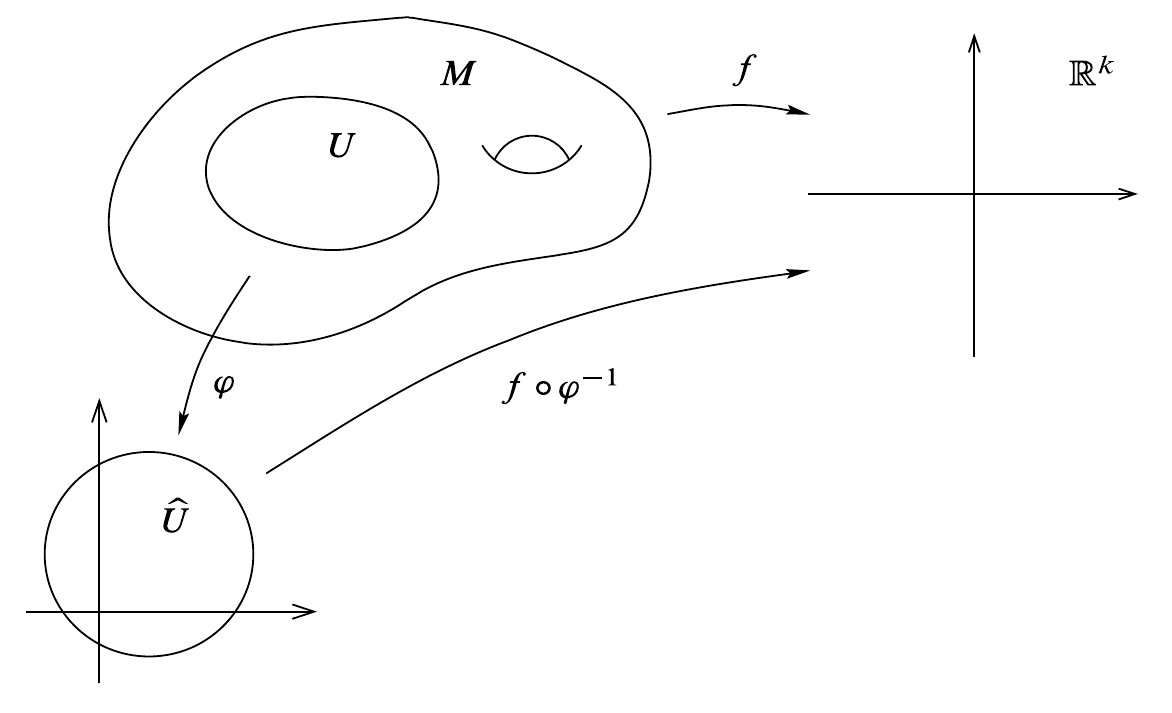
\includegraphics[scale = 0.35]{chapter02/c2f1.png}
\end{center}

\dfn Given a function $f:M\ra \Rk$ and a chart $(U,\vphi)$ for $M$, the function $\wh f:\vphi(U)\ra \Rk$ defined by $\wh f(x) = f\circ\vphi\inv(x)$ is called the \textbf{\textit{coordinate representation of f}}.

\dfn Let $M,\,N$ be smooth manifolds, and let $F:M\ra N$ be any map. We say that $F$ is a \textbf{\textit{smooth map}} if for every $p\in M$, there exist smooth charts $(U,\vphi)$ containing $p$ and $(V,\psi)$ containing $F(p)$ such that $F(U)\seq V$ and the composite map $\psi\circ\vphi\inv$ is smooth from $\vphi(U)$ to $\psi(V)$.

\begin{center}
    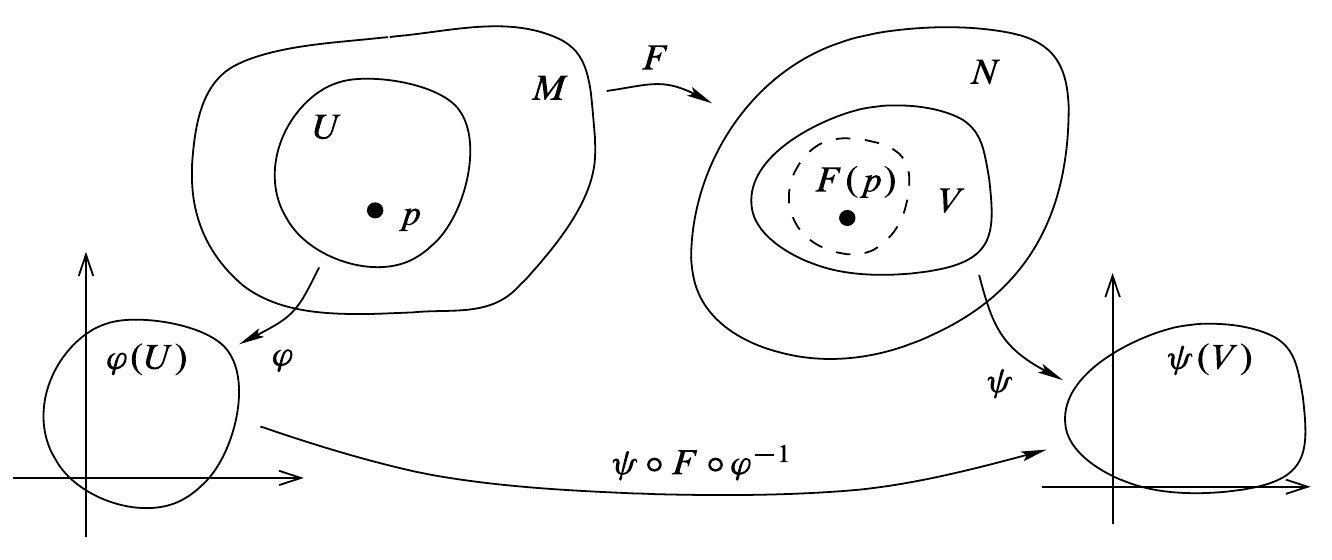
\includegraphics[scale = 0.4]{chapter02/c2f2.png}
\end{center}

\setcounter{thm}{3}

\begin{prop}
Every smooth map is continuous
\end{prop}

\begin{prop}[Equivalent Characterizations of Smoothness]
Suppose $M$ and $N$ are smooth manifolds with or without boundary, and $F:M\ra N$ is a map. Then $F$ is smooth if and only if either of the following conditions is satisfied:
\begin{enumerate}
    \item For every $p\in M$, there exist smooth charts $(U,\vphi)$ containing $p$ and $(V, \psi)$ containing $F(p)$ such that $U\cap F\inv(V)$ is open in $M$ and the composite map $\psi\circ F\circ \vphi\inv$ is smooth from $\vphi(U\cap F\inv(V))$ to $\psi(V)$.
    \item $F$ is continuous and there exist smooth atlases $\{(U_\al, \vphi_\al)\}$ and $\{(V_\be, \psi_\be)\}$ for $M$ and $N$, respectively, such that for each $\al$ and $\be$, $\psi_\be\circ F\circ\vphi_\al\inv$ is a smooth map from $\vphi_\al(U_\al\cap F\inv(V_\be))$ to $\psi_\be(V_\be)$.
\end{enumerate}
\end{prop}

\begin{prop}[Smoothness is Local]Let $M$ and $N$ be smooth manifolds with or without boundary, and let $F:M\ra N$ be a map.
\begin{enumerate}
    \item If every point $p\in M$ has a neighborhood $U$ such that the restriction $F|_U$ is smooth, then $F$ is smooth.
    \item Conversely, if $F$ is smooth, then its restriction to every open subset is smooth.
\end{enumerate}
\end{prop}

\setcounter{thm}{7}

\begin{cor}[\hl{Gluing Lemma for Smooth Maps}]
Let $M$ and $N$ be smooth manifolds with or without boundary, and let $\{U_\al\}_{\al\in A}$ be an open cover of $M$. Suppose that for each $\al\in A$, we are given a smooth map $F_\al:U_\al\ra N$ such that the maps agree on overlaps: $\ev{F_\al}{U_\al\cap U_\be} = \ev{F_\be}{U_\al\cap U_\be}$ for all $\al$ and $\be$. Then there exists a unique smooth map $F:M\ra N$ such that $\ev{F}{U_\al} = F_\al$ for each $\al\in A$.
\end{cor}

\setcounter{thm}{9}

\begin{prop}Let $M$, $N$, and $P$ be smooth manifolds with or without boundary.
\begin{enumerate}
    \item Every constant map $c:M\ra n$ is smooth.
    \item The identity map of $M$ is smooth.
    \item \hl{If $C\seq M$ is an open submanifold with or without boundary, then the inclusion map $U\into M$ is smooth.}
    \item If $F:M\ra N$ and $G:N\ra P$ are smooth, then so is $G\circ F:M\ra P$.
\end{enumerate}
\end{prop}

\setcounter{thm}{11}

\begin{prop}
Suppose $M_1,\ldots,M_k$ and $N$ are smooth manifolds with or without boundary, such that at most one of $M_1,\ldots,M_k$ has nonempty boundary. For each $i$, let $\pi_I:M_1\x \cdots\x M_k\ra M_i$ denote the projection onto the $M_i$ factor. A map $F:N\ra M_1\x \cdots \x M_k$ is smooth if and only if each of the component maps $F_i = \pi_i\circ F:N\ra M_i$ is smooth.
\end{prop}

\dfn If $M$ and $N$ are smooth manifolds with or without boundary, a \textbf{\textit{diffeomorphism from M to N}} is a smooth bijective map $F:M\ra N$ that has a smooth inverse.

\setcounter{thm}{17}

\begin{thm}[Diffeomorphism Invariance of Dimension]
A nonempty smooth manifold of dimension $m$ cannot be diffeomorphic to an $n$-dimensional smooth manifold unless $m = n$
\end{thm}

\begin{thm}[Diffeomorphism Invariance of Boundary]
Suppose $M$ and $N$ are smooth manifolds with boundary and $F:M\ra N$ is a diffeomorphism. Then $F(\bd M) = \bd N$, and $F$ restricts to a diffeomorphism from $\Int(M)$ to $\Int(N)$.
\end{thm}
\newpage
\subsection{Partitions of Unity}\nl

\begin{lem}
The functions $f:\R\ra \R$ defined by
\[f(t) = \begin{cases} e^{-\frac{1}{t}}, & t > 0,\\ 0. & t\leq 0,\end{cases}\]
is smooth.
\end{lem}

\begin{lem}
Given any real numbers $r_1$ and $r_2$ such that $r_1 < r_2$, there exists a smooth function $h:\R\ra \R$ such that $h(t) \equiv 1$ for $t\leq r_1$, $0 < h(t) < 1$ for $r_1 < t < r_2$, and $h(t) \equiv 0$ for $t\geq r_2$.
\end{lem}

\begin{proof}
Let $f$ be the function of the previous lemma, and set 
\[h(t) = \frac{f(r_2 - t)}{f(r_2 - t) + f(t - r_1)}.\]
Then the denominator is always positive since $r_2 \neq r_1$ and either $r_2 - t$ or $t - r_1$ will always be positive, and the rest follows form the properties of $f$.
\end{proof}

\begin{lem}
Given any positive real numbers $r_1 < r_2$, there is a smooth function $H:\Rn\ra \R$ such that $H \equiv 1$ on $\ol B_{r_1}(0), 0 < H(x) < 1$ for all $x \in B_{r_2}(0)\backslash \ol B_{r_1}(0)$, and $H\equiv 0$ on $\Rn \backslash B_{r_2}(0)$.
\end{lem}

\dfn The function $H$ constructed in the previous lemma is an example of a \df{smooth bump function}, a smooth real-valued function that is equal to 1 on a specified set and is zero outside a specified neighborhood of that set.

\dfn If $f$ is any real-valued or vector-valued function on a topological space $M$, the \df{support of f}, denoted $\supp(f)$, is the \ul{closure of the set of points} where $f$ is nonzero:
\[\supp(f) = \ol{\{p\in M\ :\ f(p)\neq 0\}}\]
A function $f$ is said to be \df{compactly supported} if $\supp(f)$ is a compact set.

\dfn Suppose that $M$ is a topological space, and let $\XX = (X_\al)_{\al\in A}$ be an arbitrary open cover of $M$. A \df{partition of unity subordinate to $\boldsymbol{X}$} is an indexed family $(\psi_\al)_{\al\in A}$ of continuous functions $\psi_\al:M\ra \R$ with the following properties:
\begin{enumerate}[(i)]
    \item $0 \leq \psi_\al(x)\leq 1$ for all $\al\in A$ and all $x\in M$.
    \item $\supp(\psi_\al) \seq X_\al$ for each $\al\in A$.
    \item The family of supports $(\supp(\psi_\al))_{\al\in A}$ is locally finite. 
    \item $\sum_{\al\in A}\psi_\al(x) = 1$ for all $x\in M$.
\end{enumerate}
If $M$ is a smooth manifold with or without boundary, a \df{smooth partition of unity} is one for which each of the unctions $\psi_\al$ is smooth.

\begin{thm}[Existence of Partitions of Unity]
Suppose $M$ is a smooth manifold with or without boundary, and $\XX = (X_\al)_{\al\in A}$ is any indexed open cover of $M$. Then there exists a smooth partition of unity subordinate to $\XX$.
\end{thm}

\dfn If $M$ is a topological space, $A\seq M$ is a closed subset, and $U\seq M$ is an open subset containing $A$, a continuous function $\psi:M\ra \R$ is called a \df{\hl{bump function for A supported in U}} if $0 \leq \psi \leq 1$ on $M$, $\psi \equiv 1$ on $A$, and $\supp(\psi)\seq U$.

\setcounter{thm}{24}

\begin{prop}[Existence of Smooth Bump Functions]
Let $M$ be a smooth manifold with or without boundary. For any closed subset $A\seq M$ and any open subset $U$ containing $A$, there exists a smooth bump function for $A$ supported in $U$.
\end{prop}

\dfn Suppose that $M$ and $N$ are smooth manifolds with or  without boundary, and $A\seq M$ is an arbitrary subset. We say that a map $F:A\ra N$ is \df{smooth on A} if it has a smooth extension in a neighborhood of each point: that is, if for every $p\in A$ there is an open subset $W\seq M$ containing $p$ an a smooth map $\td F:W\ra N$ whose restriction to $W\cap A$ agrees with $F$.

\begin{lem}[\hl{Extension Lemma for Smooth Functions}]
Suppose $M$ is a smooth manifold with or without boundary, $A\seq M$ a closed subset, and $f:M\ra \Rk$ is a smooth function. For any open subset $U$ containing $A$, there exists a smooth function $\td f:M\ra \Rk$ such that $\td f_A = f$ and $\supp(\td f)\seq U$.
\end{lem}

\dfn Suppose that $M$ is a topological space. An \df{exhaustion function for M} is a continuous function $f:M\ra \R$ with the property that the set $f\inv((-\infty, c])$ (called a \df{sublevel set of f}) is compact for each $c\in \R$. For an example consider the function $f:\Rn\ra \R:x\mapsto |x|^2$.

\setcounter{thm}{27}

\begin{prop}[Existence of Smooth Exhaustion Functions]
Every smooth manifold with or without boundary admits a smooth, positive exhaustion function.
\end{prop}

\begin{thm}[\hlb{Level Sets of Smooth Functions}]
Let $M$ be a smooth manifold. If $K$ is any closed subset of $M$, there is a smooth, nonnegative function $f:M\ra \R$ such that $f\inv(0) = K$.
\end{thm}











\newpage\setcounter{section}{2}
\section{Tangent Vectors}

One of the very central ideas that we have in ordinary calculus is the idea of \textit{linear approximation}. In ordinary calculus, we approximated things by funding the tangent line to some curve at a specified point. However, to make sense of this notion for smooth manifolds, we need to talk about the idea of a \textit{tangent space to a manifold at a point}. The basic principles of these objects were introduced to us back in Calculus III when we learned about tangent vectors to curves and tangent planes to surfaces, so we will use this as the starting position for our discussion of geometric tangent vectors in $\Rn$.


\dfn Given a point $a\in \Rn$, let us define the \df{geometric tangent space to $\boldsymbol{\Rn}$ at a}, denoted by $\Rn_a$, to be the set $\{a\}\x \Rn$. A \df{geometric tangent vector} in $\Rn$ is an element of $\Rn_a$ for some $a\in \Rn$.

\dfn Given any geometric tangent vector $v_a\in \Rn_a$, we can define a map $D_v|_a:\Cin(\Rn)\ra \R$, which takes the directional derivative in the direction $v$ at $a$:
\[D_v|_a f = D_vf(a) = \ev{\frac{d}{dt}}{t = 0}f(a + tv).\]
If $v_a = v^ie_i|_a$ in terms of the standard basis, then by the chain rule, we can write
\[D_v|_af = v^i\pd{f}{x^i}(a).\]

\dfn A map $w:\Cin(\Rn)\ra \R$ is called a \df{derivation at a} if it is linear over $\R$ and satisfies the Leibniz rule:
\[w(fg) = f(a)wg + g(a)wf.\]
We will denote the set of all derivations of $\Cin(\Rn)$ at $a$ by $T_a\Rn$.

\begin{lem}[Properties of Derivations]
Suppose $a\in \Rn$, $w\in T_a\Rn$, and $f,g\in \Cin(\Rn)$.
\begin{enumerate}
    \item If $f$ is a constant function, then $wf = 0$.
    \item If $f(a) = g(a) = 0$ then $w(fg) = 0$.
\end{enumerate}
\end{lem}

\begin{prop}
Let $a\in \Rn$
\begin{enumerate}
    \item For each geometric tangent vector $v_a\in \Rn_a$, the map $D_v|_a:\Cin(\Rn)\ra \R$ is a derivation at $a$.
    \item The map $v_a\mapsto D_v|_a$ is an isomorphism form $\Rn_a$ onto $T_a\Rn$.
\end{enumerate}
\end{prop}

\begin{cor}
For any $a\in \Rn$, the $n$ derivations
\[\ev{\pdd{x^1}}{a},\ldots, \ev{\pdd{x^n}}{a}\quad\text{defined by}\quad \ev{\pdd{x^i}}{a}f = \pd{f}{x^i}(a)\]
form a basis for $T_a\Rn$, which therefore has dimension $n$.
\end{cor}

With this machinery out of the way, we are ready to generalize our notion of a tangent space to an arbitrary manifold.

\newpage

\subsection{Tangent Vectors on Manifolds}\nl

\dfn Let $M$ be a smooth manifold with or without boundary, and let $p$ be a point of $M$. A linear map $v:\Cin(M)\ra \R$ is called a \df{derivation at p} if it satisfies
\[v(fg) = f(p)vg + g(p)vf\quad\text{for all }f,g\in \Cin(M)\]
The set of all derivations of $\Cin(M)$ at $p$, denoted by $T_pM$, is a vector space called the \df{tangent space to M at p}. An element of $T_pM$ is called a \df{tangent vector at p}.

\begin{lem}[Properties of Tangent Vectors on Manifolds]
Suppose $M$ is a smooth manifold with or without boundary, $p\in M$, $v\in T_pM$, and $f,g\in \Cin(M)$.
\begin{enumerate}
    \item If $f$ is a constant function, then $vf = 0$.
    \item If $f(p) = g(p) = 0$, then $v(fg) = 0$.
\end{enumerate}
\end{lem}

\dfn If $M$ and $N$ are smooth manifolds with or without boundary and $F:M\ra N$ is a smooth map, for each $p\in M$ we define a map
\[dF_p:T_pM\ra T_pN,\]
called the \df{differential of F at p}, as follows. Given $v\in T_pM$, we let $dF_p(b)$ be the derivation at $F(p)$ that acts on $f\in \Cin(N)$ by the rule
\[dF_p(v)(f) = v(f\circ F).\]

\setcounter{thm}{5}

\begin{prop}[Properties of Differentials]
Let $M,\,N$, and $P$ be smooth manifolds with or without boundary, let $F:M\ra N$ and $G:N\ra P$ be smooth maps, and let $p\in M$.
\begin{enumerate}
    \item $dF_p:T_pM\ra T_{F(p)}N$ is linear.
    \item \hl{$d(G\circ F)_p = dG_{F(p)}\circ dF_p:T_pM|raT_{G\circ F(p)}P$}
    \item $d(\Id|_M)_p = Id_{T_pM}:T_pM\ra T_pM$.
    \item \hl{If $F$ is a diffeomorphism, then $dF_p:T_pM\ra T_pN$ is an isomorphism and $(dF_p)\inv = d(F\inv)_{F(p)}$.}
\end{enumerate}
\end{prop}

\setcounter{thm}{7}

\begin{prop}
Let $M$ be a smooth manifold with or without boundary, $p\in M$, and $v\in T_pM$. If $f,g\in \Cin(M)$ agree on some neighborhood of $p$, then $vf = vg$.
\end{prop}

\begin{prop}[\hlb{The Tangent Space to an Open Submanifold}]
Let $M$ be a smooth manifold with or without boundary, let $U\seq M$ be an open subset and let $\iota:U\into M$ be the inclusion map. For every $p\in U$, the differential $d\iota_p:T_pU\ra T_pM$ is an isomorphism.
\end{prop}

\begin{prop}[Dimension of the Tangent Space]
If $M$ is an $n$-dimensional smooth manifold, then for each $p\in M$, the tangent space $T_PM$ is an $n$-dimensional vector space.
\end{prop}

\begin{lem}
Let $\iota\Hn\into \Rn$ denote the inclusion map. For any $a\in \bd \Hn$, the differential $d\iota_a:T_a\Hn\ra T_a\Rn$ is an isomorphism.
\end{lem}

\begin{prop}[Dimension of Tangent Spaces on a Manifold with Boundary]
Suppose $M$ is an $n$-dimensional smooth manifold with boundary. For each $p\in M$, $T_pM$ is an $n$-dimensional vector space.
\end{prop}

\dfn Suppose $V$ is a finite-dimensional vector space and $a\in V$. For any vector $v\in V$, we define a map $D_v|_a:\Cin(V) \ra \R$ by 
\[D_v|_a f = \ev{\frac{d}{dt}}{t=0}f(a + tv).\]

\begin{prop}[\hlb{The Tangent Space to a Vector Space}]
Suppose $V$ is a finite-dimensional vector space with its standard smooth manifold structure. For each point $a\in V$, the $v\mapsto D_v|_a$ as defined above is a canonical isomorphism from $V$ to $T_aV$, such that for any linear map $L:V\ra W$, the following diagram commutes:
\begin{center}
\begin{tikzcd}[row sep = 2em, column sep = 2em]
V\arrow[r, "\cong"]\arrow[d, swap, "L"] & T_aV\arrow[d, "dL_a"]\\
W\arrow[r, "\cong"] & T_{L_a}W
\end{tikzcd}.
\end{center}
\end{prop}

\begin{prop}[The Tangent Space to a Product Manifold]
Let $M_1,\ldots,M_k$ be smooth manifolds, and for each $j$, let $\pi_j:M_1\x\cdots\x M_k\ra M_j$ be the projection map onto the $M_j$ factor. For any point $p = (p_1,\ldots,p_k)\in M_1\x\cdots\x M_k$, the map
\[\al:T_p(M_1\x\cdots\x M_k)\ra T_{p_1} \oplus \cdots \oplus T_{p_k}M_k\]
defined by
\[\al(v) = (d(\pi_1)_p(v),\ldots,d(\pi_k)_p(v))\]
is an isomorphism. The same is true if one of the spaces $M_i$ is a smooth manifold with boundary.
\end{prop}

\subsection{Computation in Coordinates}\nl

\begin{prop}
Let $M$ be a smooth $n$-manifold with or without boundary, and let $p\in M$. Then $T_p M$ is an $n$-dimensional vector space, and for any smooth chart, $(U, (x^i))$ (where $(x^i)$ is just the coordinate representation of some chart map $\vphi$) containing p, the coordinate vectors $\pdd{x^1}|_p,\ldots,\pdd{x^n}|_p$ form a basis for $T_pM$.
\end{prop}

\dfn Any tangent vector $v\in T_pM$ can be written uniquely as a linear combination
\[v = v^i\ev{\pdd{x^i}}{p}.\]
The ordered basis $\lp\ev{\pdd{x^i}}{p}\rp$ is called a \df{coordinate basis for $\boldsymbol{T_pM}$}, and the numbers $(v^1,\ldots,v^n)$ are called the \df{components of v} with respect to the coordinate basis.

\dfn In the case where $F:U\ra V$ is a smooth map between $U\seq \Rn$ and $V\seq \Rm$ with $U$ and $V$ open subsets of Euclidean spaces with coordinates $x^1,\ldots,x^n)$ and $(y^1,\ldots, y^m)$ respectively. For any $p\in U$, we can use the chian rule to compute that the action of $dF_p$ on a typical basis vector as follows:
\[dF_p\lp \ev{\pdd{x^i}}{p}\rp f = \lp\pd{F^j}{x^i}(p) \ev{\pdd{y^j}}{F(p)}\rp f.\]
Thus
\[dF_p\lp \ev{\pdd{x^i}}{p}\rp = \pd{F^j}{x^i}(p) \ev{\pdd{y^j}}{F(p)}.\]
And this gives us that the matrix of $dF_p$ in terms of the coordinate bases is
\[\bpm \pd{F^1}{x^1}(p) & \cdots & \pd{F^1}{x^n}\\ 
       \vdots & \ddots & \vdots\\
       \pd{F^m}{x^1}(p) & \cdots & \pd{F^m}{x^n}(p)\epm.\]

\dfn For a general smooth map $F:M\ra N$ between smooth manifolds with or without boundary with coordinate charts $(U,\vphi)$ for $M$ containing some point $p$ and $(V, \psi)$ for $N$ containing $F(p)$, we obtain the coordinate representation $\wh F = \psi \circ F \circ \vphi\inv:\vphi(U\cap F\inv(V))\ra \psi(V)$. Let $\wh p = \vphi(p)$ denote the coordinate representation of $p$. By the computation above $d\wh F_{\wh p}$ is represented with respect to the standard coordinate bases by the Jacobian matrix of $\wh F$ at $\wh p$. Using the fact that $F\circ \vphi\inv = \psi \circ \wh F$, \hl{we compute that}
\[dF_p\lp\ev{\pdd{x^i}}{p}\rp = \pd{\wh F^j}{x^i}(\wh p)\ev{\pdd{y^j}}{F(p)}.\]

\begin{center}
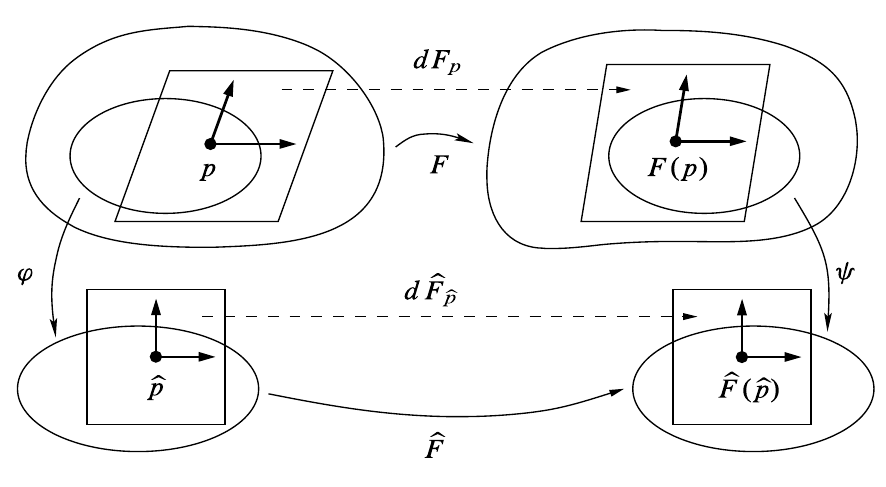
\includegraphics[scale = 0.5]{chapter03/c3f6.png}
\end{center}

\hl{\textbf{Note:}} In the differential geometry literature, the differential is sometimes called the \df{tangent map}, the \df{total derivative}, or simply the \df{derivative of F}. It can also sometimes be called the \df{(pointwise) pushforward}. Different authors denote it using symbols such as
\[F\p(p),\quad DF,\quad DF(p),\quad F_*,\quad TF, \quad T_pF.\]
However, we will stick to the notation $dF_p$.

\dfn Suppose $(U,\vphi)$ and $(V,\psi)$ are two smooth charts on $M$, and $p\in U\cap V$. Let us denote the coordinate functions of $\vphi$ by $(x^i)$ and those of $\psi$ by $(\td x^i)$. Then any tangent vector at $p$ can be represented with respect to either basis $\lp\ev{\pdd{x^i}}{p}\rp$ or $\lp\ev{\pdd{\td x^i}}{p}\rp$. Using our transition map and the definition of coordinate vectors, \hl{we can compute that}
\[\ev{\pdd{x^i}}{p} = \pd{\td x^j}{x^i}(\wh p)\ev{\pdd{\td x^j}}{p}.\]

\begin{ex}[\hlo{Polar Coordinates}]
The transition map between polar coordinates and standard coordinates in suitable open subsets of the plane is given by $(x,y) = (r\cos(\theta),r\sin(\theta)$. Let $p = (r,\theta) = (2, \pi/2)$, and let $v\in T_p\R^2$ be the tangent vector whose polar coordinate representation is
\[v = 3\ev{\pdd{r}}{p} = \ev{\pdd{\theta}}{p}.\]
Applying the rule in the above definition, we get that
\begin{align*}
    \ev{\pdd{r}}{p} &= \cos\lp\frac{\pi}{2}\rp\ev{\pdd{x}}{p} + \sin\lp\frac{\pi}{2}\rp\ev{\pdd{y}}{p} = \ev{\pdd{y}}{p},\\
    \ev{\pdd{\theta}}{p} &= 
    -2\sin\lp\frac{\pi}{2}\rp\ev{\pdd{x}}{p} + 2\cos\lp\frac{\pi}{2}\rp\ev{\pdd{y}}{p} = -2\ev{\pdd{x}}{p},
\end{align*}
and thus $v$ has the following coordinate representation in standard coordinates:
\[v = 3\ev{\pdd{y}}{p} + 2\ev{\pdd{x}}{p}.\]
\end{ex}


\subsection{The Tangent Bundle}\nl

\dfn Given a smooth manifold $M$ with or without boundary, we define the \df{tangent bundle of M}, denoted by $TM$, to be the disjoint union of the tangent spaces at all points of $M$:
\[TM = \bigsqcup_{p\in M} T_pM.\]

\nb We usually write an element of this disjoint union as an ordered pair $(p,v)$ with $p\in M$ and $v\in T_pM$, and the tangent bundle comes equipped with a natural projection map $\pi:TM\ra M:(p,v)\mapsto p$.

\setcounter{thm}{17}

\begin{prop}
For any smooth $n$-manifold $M$, the tangent bundle $TM$ has a natural topology and a smooth structure that make it into a $2n$-dimensional smooth manifold. With respect to this structure, the projection $\pi:TM\ra M$ is smooth.
\end{prop}

\begin{center}
    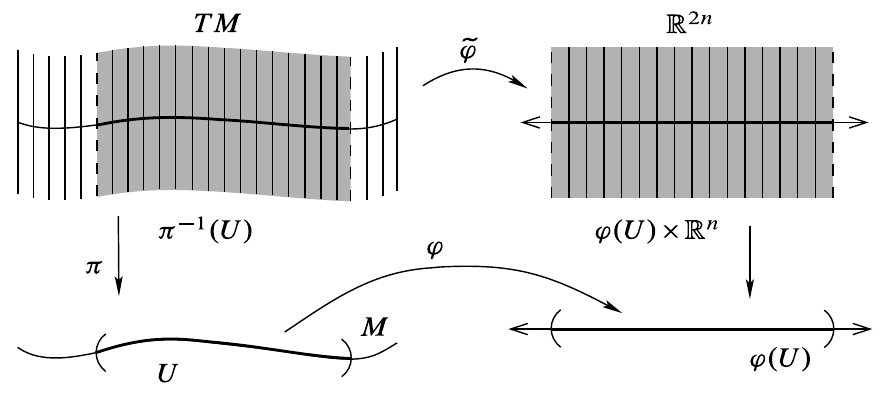
\includegraphics[scale = 0.5]{chapter03/c3f8.png}
\end{center}

\setcounter{thm}{19}

\begin{prop}
If $M$ is a smooth $n$-manifold with or without boundary, and $M$ can be covered by a single smooth chart, then $TM$ is diffoemorphic to $M\x \Rn$.
\end{prop}

\begin{prop}
If $F:M\ra N$ is a smooth map, then its global differential $dF:TM\ra TN$ is a smooth map.
\end{prop}

\begin{cor}[\hl{Properties of the Global Differential}]
Suppose $F:M\ra N$ and $G:N\ra P$ are smooth maps
\begin{enumerate}
    \item $d(G\circ F) = dG\circ dF$.
    \item $d(\Id_M) = \Id_{TM}$
    \item If $F$ is a diffeomorphism, then $dF:TM\ra TN$ is also a diffeomorphism, and $(dF)\inv = d(F\inv)$.
\end{enumerate}
\end{cor}

\dfn If $M$ is a manifold, a \df{curve in M} is a continuous map $\ga:J\ra M$, where $J\seq \R$ is an interval.

\dfn Given a smooth curve $\ga:J\ra M$, and $t_0\in J$, we define the \df{velocity of $\boldsymbol{\ga}$ at $\boldsymbol{t_0}$}, denoted by $\ga\p(t_0)$, to be the vector
\[\ga\p(t_0) = d\ga\lp\ev{\frac{d}{dt}}{t_0}\rp\in T_{\ga(t_0)}M,\]
where $\ev{\frac{d}{dt}}{t_0}$ is the standard coordinate basis vector in $T_{t_0}\R$.

\dfn Given a smooth chart $(U,(x^i))$ with $\ga(t_0)\in U$, we can write the coordinate representation of $\ga$ as $\ga(t) = (\ga^1(t),\ldots,\ga^n(t))$. Then the coordinate formula for the differential yields
\[\ga\p(t_0) = \frac{d\ga^i}{dt}(t_0)\ev{\pdd{x^i}}{\ga(t_0)}.\]

\begin{prop}
\hlb{Suppose $M$ is a smooth manifold with or without boundary and $p\in M$. Every $v\in T_pM$ is the velocity vector of some smooth curve in $M$.}
\end{prop}

\begin{prop}[The Velocity of a Composite Curve]
Let $F:M\ra N$ be a smooth map, and let $\ga:J\ra M$ be a smooth curve. For any $t_0\in J$, the velocity at $t = t_0$ of the composite curve $F\circ \ga:J\ra N$ is given by
\[(F\circ \ga)\p(t_0) = dF(\ga\p(t_0)).\]
\end{prop}

\begin{cor}[Computing the Differential Using a Velocity Vector]
Suppose $F:M\ra N$ is a smooth map, $p\in M$, and $v\in T_pM$. Then 
\[dF_p(v) = (F\circ \ga)\p(0)\]
for any smooth curve $\ga:J\ra M$ such that $0\in J, \ga(0) = p$, and $\ga\p(0) = v$.
\end{cor}







\newpage\setcounter{section}{3}
\section{Submersions, Immersions, and Embeddings}

We now have a way of giving the "best linear approximation" of a map near a given point on a manifold However, we can learn a great deal about a map by studying the properties of its differential, and that's exactly what we do in this section. Many of the properties of smooth submersions and smooth immersions that we study in this chapter will form the basis for our understanding of submanifolds which we will explore in the next chapter.

\subsection{Maps of Constant Rank}\nl

\dfn Suppose $M$ and $N$ are smooth manifolds with or without boundary. Given a smooth map $F:M\ra N$ and a point $p\in M$, we define the \df{rank of F at p} to be the rank of the linear map $dF_p:T_pM\ra T_{F(p)}N$; it is the rank of the Jacobian matrix of $F$ in any smooth chart. If $F$ has rank $r$ at every point, we say that it has \df{constant rank}, and write $\rank(F) = r$.

\nb $\rank(F) \leq \min\{\dim(M),\dim(N)\}$

\dfn If $\rank(dF_p) = \min\{\dim(M),\dim(N)\}$ then we way that \df{F has full rank at p}, and if $F$ has full rank everywhere, we say that \df{F has full rank}.

\dfn $F:M\ra N$ is called a \df{smooth submersion} if its differential is surjective at each point ($\rank(F) = \dim(N)$) and is called a \df{smooth immersion} if its differential is injective at each point ($\rank(F) = \dim(M)$).

\begin{prop}
Suppose $F:M\ra  N$ is a smooth map and $p\in M$. If $dF_p$ is surjective, then $p$ has a neighborhood $U$ such that $F|_U$ is a submersion. If $dF_p$ is injective, then $p$ has a neighborhood $U$ such that $F|_U$ is an immersion.
\end{prop}

\dfn If $M$ and $N$ are smooth manifolds with or without boundary, a map $F:M\ra N$ is called a \df{local diffeomorphism} if every point $p\in M$ has a neighborhood $U$ such that $F(U)$ is open in $N$ and $F|_U:U\ra F(U)$ is a diffeomorphism.

\setcounter{thm}{4}

\begin{thm}[\hlb{Inverse Function Theorem for Manifolds}]
Suppose $M$ and $N$ are smooth manifolds, and $F:M\ra N$ is a smooth map. If $p\in M$ is a point such that $dF_p$ is invertible, then there are connected neighborhoods $U_0$ of $p$ and $V_0$ of $F(p)$ such that $F|_{U_0}:U_0\ra V_0$ is a diffeomorphism.
\end{thm}

\setcounter{thm}{7}

\begin{prop}
Suppose $M$ and $N$ are smooth manifolds (without boundary), and $F:M\ra N$ is a map.
\begin{enumerate}
    \item $F$ is a local diffeomorphism if and only if it is both a smooth immersion and a smooth submersion.
    \item If $\dim(M) = \dim(N)$ and $F$ is either a smooth immersion or a smooth submersion, then it is a local diffeomorphism.
\end{enumerate}
\end{prop}

\setcounter{thm}{11}

\begin{thm}[\hlb{Rank Theorem}]
Suppose $M$ and $N$ are smooth manifolds of dimensions $m$ and $n$, respectively, and $F:M\ra N$ is a smooth map \hl{with constant rank} $r$. For each $p\in M$ there exist smooth charts $(U,\vphi)$ for $M$ centered at $p$ and $(V,\psi)$ for $N$ centered at $F(p)$ such that $F(U)\seq V$, in which $F$ has a coordinate representation of the form
\[\wh F(x^1,\ldots,x^r,x^{r+1},\dots x^m) = (x^1,\ldots,x^r,0,\ldots,0).\]
In particular, if $F$ is a smooth submersion, this becomes
\[\wh F(x^1,\ldots,x^n,x^{n+1},\dots x^m) = (x^1,\ldots,x^n),\]
and if $F$ is a smooth immersion, it is
\[\wh F(x^1,\ldots, x^m) = (x^1,\ldots,x^m,0,\ldots,0).\]
\end{thm}

\begin{cor}
Let $M$ and $N$ be smooth manifolds, let $F:M\ra N$ be a smooth map, and suppose $M$ is connected. Then the following are equivalent:
\begin{enumerate}
    \item For each $p\in M$ there exist smooth charts containing $p$ and $F(p)$ in which the coordinate representation of $F$ is linear.
    \item $F$ has constant rank.
\end{enumerate}
\end{cor}


\begin{thm}[Global Rank Theorem]
Let $M$ and $N$ be smooth manifolds, and suppose $F:M\ra N$ is a smooth map of constant rank.
\begin{enumerate}
    \item If $F$ is surjective, then it is a smooth submersion.
    \item If $F$ is injective, then it is a smooth immersion.
    \item If $F$ is bijective, then it is a diffeomorphism.
\end{enumerate}
\end{thm}

\subsection{Embeddings and Submersions}\nl

\dfn If $M$ and $N$ are smooth manifolds with or without boundary, a \df{smooth embedding of M into N} is a smooth immersion $F:M\ra N$ that is also a topological embedding (i.e. a homeomorphism onto its image in the subspace topology).

\setcounter{thm}{17}

\begin{ex}[A Smooth Topological Embedding]
The map $\ga:\R\ra\R^2$ given by $\ga(t) = (t^3,0)$ is a smooth map and a topological embedding, but it is not a smooth embedding because $\ga\p(0) = 0$.
\end{ex}

\begin{ex}[The Figure-Eight Curve]
Consider the curve $\be:(-\pi,\pi)\ra \R^2:t\ra (\sin(2t), \sin(t)).$ The image is a set that looks like a figure-eight in the plane. It is easy to see that $\be$ is an injective smooth immersion because $\be\p(t)$ never vanishes; but it is not a topological embedding, because its image is compact in the subspace topology, while its domain is not.
\end{ex}

\setcounter{thm}{21}

\dfn If $X$ and $Y$ are topological spaces, a map $F:X\ra Y$ is said to be \df{\hlb{proper}} if for every compact set $K\seq Y$, the preimage $F\inv(K)$ is compact

\begin{prop}
Suppose $M$ and $N$ are smooth manifolds with or without boundary, and $F:M\ra N$ is an injective smooth immersion. \hlb{If any of the following holds, then $F$ is a smooth embedding.}
\begin{enumerate}
    \item $F$ is an open or closed map
    \item $F$ is a proper map.
    \item $M$ is compact.
    \item $M$ has empty boundary and $\dim(M) = \dim(N)$.
\end{enumerate}
\end{prop}

\setcounter{thm}{24}

\begin{thm}[\hl{Local Embedding Theorem}]
Suppose $M$ and $N$ are smooth manifolds with or without boundary, and $F:M\ra N$ is a smooth map. Then $F$ is a smooth immersion if and only if every point in $M$ has a neighborhood $U\seq M$ such that $F|_U:U\ra N$ is a smooth embedding.
\end{thm}

\dfn If $\pi:M\ra N$ is any continuous map, a \df{section of $\boldsymbol{\pi}$} is a continuous right inverse for $\pi$, i.e., a continuous map $\sigma:N\ra M$ such that $\pi\circ \sig = \Id_N$.
\begin{center}
\begin{tikzcd}
M\arrow[d, swap, "\pi"]\\ N\arrow[u, bend right, swap, "\sigma"]
\end{tikzcd}
\end{center}
A \df{local section of $\boldsymbol{\pi}$} is a continuous map $\sig:Y\ra M$ defined on some open subset $U\seq N$ and satisfying the analogous relation $\pi\circ\sigma = \Id_U$.

\begin{thm}[Local Section Theorem]
Suppose $M$ and $N$ are smooth manifolds and $\pi:M\ra N$ is a smooth map. Then $\pi$ is a smooth submersion if an only if every point of $M$ is in the image of a smooth local section of $\pi$.
\end{thm}

\dfn If $\pi:X\ra Y$ is a continuous map, we say $\pi$ is a \df{topological submersion} if ever point of $X$ is in the image of a (continuous) local section of $\pi$.

\setcounter{thm}{27}

\begin{thm}[Properties of Smooth Submersions]
Let $M$ and $N$ be smooth manifolds, and suppose $\pi:M\ra N$ is a smooth submersion. Then $\pi$ is an open map, and if it is surjective, it is a quotient map.
\end{thm}

\begin{thm}[Characteristic Property of Surjective Smooth Submersions]
Suppose $M$ and $N$ are smooth manifolds, and $\pi:M\ra N$ is a surjective smooth submersion. For any smooth manifold $P$ with or without boundary, a map $F:N\ra P$ is smooth if and only if $F\circ \pi$ is smooth:
\begin{center}
\begin{tikzcd}
M\arrow[d, swap, "\pi"]\arrow[dr, "F\circ \pi"] & \\ N\arrow[r, swap,  "F"] & P.
\end{tikzcd}
\end{center}
\end{thm}

\begin{thm}[Passing Smoothly to the Quotient]
Suppose $M$ and $N$ are smooth manifolds, and $\pi:M\ra N$ is a surjective smooth submersion. If $P$ is a smooth manifold with or without boundary and $F:M\ra P$ is a smooth map that is constant on the fibers of $\pi$, then there exists a unique smooth map $\td F:N\ra P$ such that $\td F\circ \pi = F$.
\end{thm}

\begin{thm}[Uniqueness of Smooth Quotients]
Suppose $M$, $N_1$, and $N_2$ are smooth manifolds, and $\pi_1:M\ra N_1$ and $\pi_2:M\ra N_2$ are surjective smooth submersions that are constant on each other's fibers. Then there exists a unique diffeomorphism $FM_1\ra N_2$ such that $F\circ \pi_1 = \pi_2$
\begin{center}
\begin{tikzcd}[column sep = 0.5em]
 & M\arrow[dl, swap, "\pi_1"]\arrow[dr, "\pi_2"] &  \\ N_1 \arrow[rr, dashed, swap, "F"] &  & N_2
\end{tikzcd}
\end{center}
\end{thm}

\newpage\setcounter{section}{4}
\section{Submanifolds}

The bulk of this chapter will be focused on the most important type of submanifolds: embedded submanifolds. There have the subspace topology inherited from their containing manifold, and turn out to be exactly the images of smooth embeddings. The other type of submanifold we will discuss, immersed submanifolds, are slightly less nice objects since they are not required to have the subspace topology, but as you would expect, they appear as the images of injective immersions.

\subsection{Embedded and Immersed Submanifolds}\nl

\dfn An \df{embedded submanifold of M} is a subset $S\seq M$ that is a manifold in the subspace topology, endowed with a smooth structure with respect to which the inclusion map $S\into M$ is a smooth embedding. Embedded submanifolds are also called \df{regular submanifolds} by some.

\dfn If $S$ ins an embedded submanifold of $M$, the \df{codimension of S in M} is given by $\dim(M) - \dim(S)$. $M$ is called the \df{ambient manifold} for $S$, and an embedded submanifold of codimension one is called an \df{embedded hypersurface}.

\begin{prop}[Open Submanifolds]
Suppose $M$ is a smooth manifold. The embedded submanifolds of codimension 0 in $M$ are exactly the open submanifolds.
\end{prop}

\begin{prop}[Images of Embeddings as Submanifolds]
Suppose $M$ is a smooth manifold with or without boundary, $N$ is a smooth manifold, and $F:N\ra M$ is a smooth embedding. Let $S = F(N)$. With the subspace topology, $S$ is a topological manifold, and it has a unique smooth structure making it into an embedded submanifold of $M$ with the property that $F$ is a diffeomorphism onto its image.
\end{prop}

\setcounter{thm}{3}

\begin{prop}[Graphs as Submanifolds]
Suppose $M$ is a smooth $m$-manifold (without boundary), $N$ is a smooth $n$-manifold with or without boundary, $U\seq M$ is open, and $f:U\ra N$ is a smooth map. Let $\Gamma(f)\seq M\times N$ denote the graph of $f$:
\[\Ga(f) = \{(x,y)\in M\x N\ :\ x\in U, y = f(x)\}.\]
Then $\Ga(f)$ is an embedded $m$-dimensional submanifold of $M\x N$.
\end{prop}

\begin{center}
    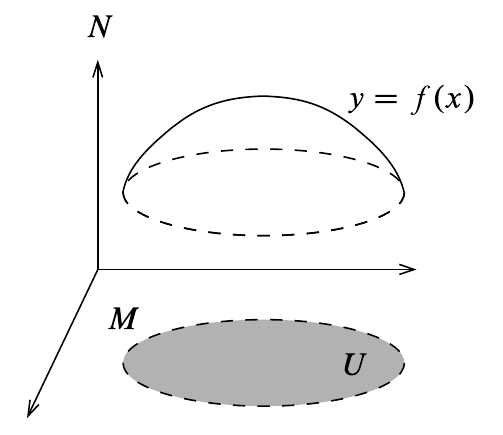
\includegraphics[scale = 0.5]{chapter05/c5f1.png}
\end{center}

\dfn An embedded submanifold $S\seq M$ is said to be \df{properly embedded} if the inclusion $S\into M$ is a proper map.

\begin{prop}
Suppose $M$ is a smooth manifold \wowob and $S\seq M$ is an embedded submanifold. Then $S$ is properly embedded if and only if it is a closed subset of $M$.
\end{prop}

\begin{cor}
Every compact embedded submanifold is properly embedded.
\end{cor}

\dfn If $Y$ is an open subset of $\Rn$ and $k\in \{0,\ldots,n\}$, a \df{k-dimensional slice of U} (or simply a \df{k-slice}) is any subset of the form 
\[S = \{(x^1,\ldots,x^k,x^{k + 1},\ldots, x^n)\in U\ :\ x^{k + 1} = c^{k + 1},\ldots,x^n = c^n\}\]
for some constants $c^{k + 1},\ldots,c^n$.

\dfn Let $M$ be a smooth $n$-manifold, and let $(U,\vphi)$ be a smooth chart on $M$. If $S$ is a subset of $U$ such that $\vphi(S)$ is a $k$-slice of $\vphi(U)$, the we say that \df{S is a k-slice of U}.

\dfn Given a subset $S\seq M$ and a nonnegative integer $k$, we say that $S$ satisfies the \df{\hlb{local k-slice condition}} if each point of $S$ is contained in the domain of a smooth chart $(U, \vphi)$ for $M$ such that $S\cap U$ is a single $k$-slice in $U$. Any such chart is called a \df{slice chart for S in M}, and the corresponding coordinates $(x^1,\ldots,x^n)$ are called \df{slice coordinates}.

\setcounter{thm}{7}

\begin{thm}[\hlb{Local Slice Criterion for Embedded Submanifolds}]
Let $M$ be a smooth $n$-manifold. If $S\seq M$ is an embedded $k$-dimensional submanifold, then $S$ satisfies the local $k$-slice condition, then with the subspace topology, $S$ is a topological manifold of dimension $k$, and it has a smooth structure making it into a $k$-dimensional embedded submanifold of $M$.
\end{thm}

\begin{ex}[Spheres as Submanifolds]
For any $n\geq 0$, $\BSN$ is an embedded submanifold of $\R^{n + 1}$, because it is locally the graph of a smooth function: as is shown in Example 1.4 of Lee, the intersection of $\BSN$ with the open subset $\{x\ :\ x^i > 0\}$ is the graph of the smooth function
\[x^i = f(x^1, \ldots, x^{i - 1}, x^{i + 1}, \ldots, x^{n + 1}),\]
where $f:\B^n\ra \R$ is given by $f(u) = \sqrt{1 - |u|^2}$. Similarly, the intersection of $\BSN$ with $\{x\ :\ x^i < 0\}$ is the graph of $-f$. Since every point in $\BSN$ is in one of these sets, $\BSN$ satisfies the local $n$-slice condition and is thus an embedded submanifold of $\R^{n + 1}$. The smooth structure thus induced on $\BSN$ is the same as the one we defined in Chapter 1: in fact, the coordinates for $\BSN$ determined by these slice charts are exactly the graph coordinates defined in Example 1.31 of Lee.
\end{ex}

\setcounter{thm}{10}

\begin{thm}
If $M$ is a smooth $n$-manifold with boundary, then with the subspace topology, $\bd M$ is a topological $(n - 1)$-dimensional manifold (without boundary), and has a smooth structure such that it is a properly embedded submanifold of $M$.
\end{thm}

\dfn If $\Phi:M\ra N$ is any map and $c$ is any point of $N$, we call the set $\Phi\inv(c)$ a \df{level set of $\boldsymbol{\Phi}$}.

\setcounter{thm}{11}

\begin{thm}[\hlb{Constant-Rank Level Set Theorem}]
Let $M$ and $N$ be smooth manifolds, and let $\Phi:M\ra N$ be a smooth map with constant rank $r$. Each level set of $\Phi$ is a properly embedded submanifold of codimension $r$ in $M$.
\end{thm}

\begin{cor}[Submersion Level Set Theorem]
If $M$ and $N$ are smooth manifolds and $\Phi:M\ra N$ is a smooth submersion, then each level set of $\Phi$ is a properly embedded submanifold whose codimension is equal to the dimension of $N$.
\end{cor}

\dfn If $\Phi:M\ra N$ is a smooth map, a point $p\in M$ is said to be a \df{regular point of $\boldsymbol{\Phi}$} if $d\Phi_p:T_pM\ra T_{\Phi(p)}N$ is surjective; it is a \df{critical point of $\boldsymbol{\Phi}$} otherwise.

\dfn A point $c\in N$ is said to be a \df{regular value of $\boldsymbol{\Phi}$} if every point of the level set $\Phi\inv(c)$ is a regular point, and a\df{critical value} otherwise. In particular, if $\Phi\inv(c) = \es$, then $c$ is a regular value. Finally, a level set $\Phi\inv(c)$ is called a \df{regular level set} if $c$ is a regular value of $\Phi$.

\begin{cor}[\hlb{Regular Level Set Theorem}]
Every regular level set of a smooth map between smooth manifolds is a properly embedded submanifold whose codimension is equal to the dimension of the codomain.
\end{cor}

\begin{ex}[\hlo{Spheres}]
Now we can give a much easier proof that $\BSN$ is an embedded submanifold of $\R^{n + 1}$. The sphere is a regular level set of the smooth function $f:\R^{n + 1}\ra R$ given by $f(x) = |x|^2$, since $df_x(v) = 2\sum_ix^iv^i$, which is surjective except at the origin.
\end{ex}

\begin{prop}
Let $S$ be a subset of a smooth $m$-manifold $M$. Then $S$ is an embedded $k$-submanifold of $M$ if and only if every point of $S$ has a neighborhood $U$ in $M$ such that $U\cap S$ is a level set of a smooth submersion $\Phi:U\ra \R^{m - k}$.
\end{prop}

\begin{center}
    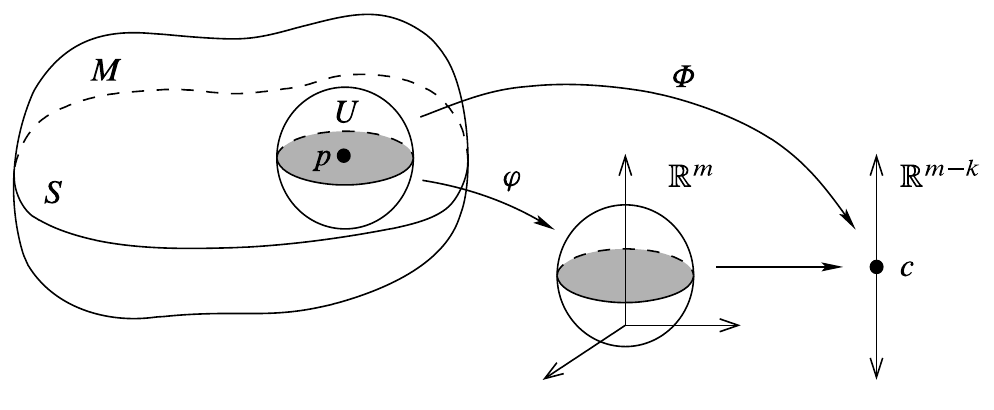
\includegraphics[scale = 0.43]{chapter05/c5f6.png}
\end{center}

\dfn If $S\seq M$ is an embedded submanifold, a smooth map $\Phi:M\ra N$ such that $S$ is a regular level set of $\Phi$ is called a \df{defining map for S}. More generally, if $U$ is an open subset of $M$ and $\Phi:U\ra N$ is a smooth map such that $S\cap U$ is a regular level set of $\Phi$, the $\Phi$ is called a \df{local defining map for S}.

\dfn An \df{\hl{immersed submanifold of M}} is a subset $S\seq M$ endowed with a topology with respect to which it is a topological manifold (without boundary), and a smooth structure with respect to which the inclusion map $S\into M$ is a smooth immersion. As for embedded submanifolds, we define the \df{codimension of S in M} to be $\dim(M) - \dim(S)$.

\setcounter{thm}{17}

\begin{prop}[\hl{Images of Immersions as Submanifolds}]
Suppose $M$ is a smooth manifold \wowob, $N$ is a smooth manifold, an d$F:N\ra M$ is an injective smooth immersion. Let $S = F(N)$. Then $S$ has a unique topology and smooth structure such that it is a smooth submanifold of $M$ and such that $F:N\ra S$ is a diffeomorphism onto its image.
\end{prop}

\setcounter{thm}{20}

\begin{prop}
Suppose $M$ is a smooth manifold \wowob, and $S\seq M$ is an immersed submanifold. If any of the following holds, then $S$ is embedded.
\begin{enumerate}
    \item $S$ has codimension 0 in $M$.
    \item The inclusion map $S\seq M$ is proper.
    \item $S$ is compact.
\end{enumerate}
\end{prop}

\begin{prop}[Immersed Submanifolds Are Locally Embedded]
If $M$ is a smooth manifold with or without boundary, and $S\seq M$ is an immersed submanifold, then for each $p\in S$ there exists a neighborhood $U$ of $p$ in $S$ that is an embedded submanifold of $M$.
\end{prop}

\dfn Suppose $X\seq M$ is an immersed $k$-dimensional submanifold. A \df{local parameterization of S} is a continuous map $X:U\ra M$ whose domain is an open subset $U\seq \Rk$, whose image is an open subset of $S$, and which, considered as a map into $S$, is a homeomorphism onto its image. It is called a \df{smooth local parameterization} if it is a diffeomorphism onto its image. If the image of $X$ is all of $S$, it is called a \df{global parameterization}.

\begin{prop}
Suppose $M$ is a smooth manifold with or without boundary, $S\seq M$ is an immersed $k$-submanifold, $\iota:S\into M$ is the inclusion map, and $U$ is an open subset of $\Rk$. A map $X:U\ra M$ is a smooth local parameterization of $S$ if and only if there is a smooth coordinate chart $(V,\vphi)$ for $S$ such that $X = \iota\circ\vphi\inv$. \hl{Therefore, every point of $S$ is the image of some local parametrization.}
\end{prop}

\setcounter{thm}{26}

\begin{thm}[Restricting the Domain of a Smooth Map]
If $M$ and $N$ are smooth manifold with or without boundary, $F:M\ra N$ is a smooth map, and $S\seq M$ is an immersed or embedded submanifold, then $F|_S:S\ra N$ is smooth.
\end{thm}

\setcounter{thm}{28}

\begin{thm}[Restricting the Codomain of a Smooth Map]
Suppose $M$ is a smooth manifold (without boundary), $S\seq M$ is an immersed submanifold, and $F:N\ra M$ is a smooth map whose image is contained in $S$. If $F$ is continuous as a map from $N$ to $S$, then $F:N\ra S$ is smooth.
\end{thm}

\begin{center}
    \includegraphics[scale = 0.38]{chapter05/c5f9.png}
\end{center}

\begin{cor}[\hl{Embedded Case}]
Let $M$ be a smooth manifold and $S\seq M$ be an embedded submanifold. Then every smooth map $F:N\ra M$ whose image is contained in $S$ is also a smooth map from $N$ to $S$.
\end{cor}

\begin{thm}
Suppose $M$ is a smooth manifold and $S\seq M$ is an embedded submanifold. \hl{The subspace topology on $S$ and the smooth structure described in Theorem 5.8 are the only topology and smooth structure with respect to which $S$ is an embedded or immersed submanifold.}
\end{thm}

\begin{thm}
Suppose $M$ is a smooth manifold and $S\seq M$ is an immersed submanifold. For the given topology on $S$, there is only one smooth structure making $S$ into an immersed submanifold.
\end{thm}

\setcounter{thm}{33}

\begin{lem}[\hlb{Extension Lemma for Functions on Submanifolds}]
Suppose $M$ is a smooth manifold, $S\seq M$ is a smooth submanifold, and $f\in \Cin(S)$.
\begin{enumerate}
    \item If $S$ is embedded, then there exists a neighborhood $U$ of $S$ in $M$ and smooth function $\td f\in \Cin(U)$ such that $\td f|_S = f$.
    \item If $S$ is properly embedded, then the neighborhood $U$ in part (a) can be taken to be all of $M$.
\end{enumerate}
\end{lem}

\newpage
\subsection{Tangent Space to a Submanifold}\nl

\dfn Let $M$ be a smooth manifold with or without boundary, and let $S\seq M$ be an immersed or embedded submanifold. Since the inclusion map $\iota:S\into M$ is a smooth immersion, at each point $p\in S$ we have an injective linear map $d\iota_p:T_pS \ra T_pM$. We adopt the convention of identifying $T_pS$ with its image under this map, thereby thinking of $T_pS$ as a certain linear subspace of $T_pM$.

\begin{center}
    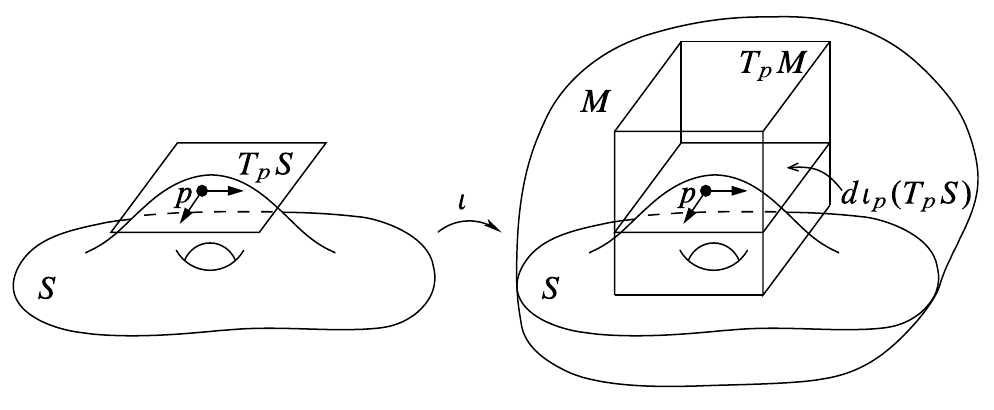
\includegraphics[scale = 0.45]{chapter05/c5f12.png}
\end{center}

\begin{prop}
Suppose $M$ is a smooth manifold \wowob, $S\seq M$ is an immersed or embedded submanifold, and $p\in S$. A vector $v\in T_pM$ is in $T_pS$ if and only if there is a smooth curve $\ga:J\ra M$ whose image is contained in $S$, and which is also smooth as a map into $S$, such that $0\in J,\ga(0) = p$, and $\ga\p(0) = v$.
\end{prop}

\setcounter{thm}{36}

\begin{prop}
Suppose $M$ is a smoth manifold, $S\seq M$ is an embedded submanifold, and $p\in S$. As a subspace of $T_pM$, the tangent space $T_pS$ is characterized by
\[T_pS = \{v\in T_pM\ :\ vf = 0\text{ whenever $f\in \Cin(M)$ and }f|_S = 0\}.\]
\end{prop}

\begin{prop}
Suppose $M$ is a smooth manifold and $S\seq M$ is an embedded submanifold. If $\Phi:U\ra N$ is any local defining map for $S$, then $T_pS = \ker(d\Phi_p):T_pM\ra T_{\Phi(p)}N$ for each $p\in S\cap U$.
\end{prop}

\begin{cor}
Suppose $S\seq M$ is a level set of a smooth submersion $\Phi = (\Phi^1,\ldots,\Phi^k):M\ra \Rk$. A vector $v\in T_pM$ is tangent to $S$ if and only if $v\Phi^1= \cdots = v\Phi^k = 0$.
\end{cor}


\hlb{\textbf{Note:}} In general there are several good strategies for showing $S\seq M$ is \textit{not} an immersed. Here are some useful facts to keep in mind:
\begin{enumerate}
    \item If $S$ is immersed, then $T_pS$ is a linear subspace of $T_pM$ of the same dimension at every $p\in S$
    \item Every $p\in S$ must be the image of some local parameterization $X:U\ra S$.
    \item Every $v\in T_pS$ is the velocity vector of some curve in $S$.
    \item \hl{Every tangent vector of $S$ annihilates every smooth function on $M$ that is constant on $S$.}
\end{enumerate}
\newpage\setcounter{section}{5}
\section{Sard's Theorem}

This chapter is a big 'ol collection of odds and ends that are useful for the prelim exam. The first part will just be talking about some theorems that are really important in Algebraic Topology and will be used later in the proofs of some important theorems. The second part, however, contains the more important material relating to transverse submanifolds.

\subsection{Sard and Whitney}

\setcounter{thm}{9}

\begin{thm}[Sard's Theorem]
Suppose $M$ and $N$ are smooth manifolds \wowob and $F:M\ra N$ is a smooth map. Then the set of critical values of $F$ has measure zero in $N$.
\end{thm}

\begin{cor}
Suppose $M$ and $N$ are smooth manifolds \wowob, and $F:M\ra N$ is a smooth map. If $\dim(M) < \dim(N)$, then $F(M)$ has measure zero in $N$.
\end{cor}

\begin{thm}[Whitney Embedding Theorem]
Every smooth $n$-manifold \wowob admits a proper smooth embedding into $\R^{2n + 1}$.
\end{thm}

\nb Just because you can, doesn't mean that you should.

\setcounter{thm}{20}

\begin{thm}[\hlb{Whitney Approximation Theorem}]
Let $M$ be a smooth manifold \wowob. If $F:M\ra \Rk$ is continuous, then given any positive continuous function $\de:M\ra \R$, there exists a smooth function $\td F$ such that $|F(x) - \td F(x)|< \de(x)$ for all $x\in M$. Furthermore, if $F$ is smooth on a closed subset, then $\td F$ can be chosen to agree with $F$ on that set.
\end{thm}

\dfn If $M$ is a $m$-dimensional embedded submanifold of $\Rn$ then the \df{normal bundle of M} is defined to be 
\[NM = \{(x,v)\in T\Rn\cong \Rn\x\Rn\ :\ x\in M,v\in T_x\Rn\ s.t.\,\,\, v\cdot w = 0 \,\,\,\forall w\in T_xM\}\]

\setcounter{thm}{22}

\begin{thm}
If $M\seq \Rn$ is an embedded $m$-dimensional submanifold, then $NM$ is an embedded $n$-dimensional submanifold of $T\Rn \cong \Rn\x\Rn$.
\end{thm}

\dfn Thinking of $NM$ as a submanifold of $\Rn\x\Rn$, we define $E:NM\ra \Rn$ by
\[E(x,v) = x + v.\]

\dfn If $M\seq \Rn$ is an embedded $m$-dimensional submanifold, a \df{tubular neighborhood of M} is a neighborhood $U$ of $M$ in $\Rn$ that is the diffeomorphic image under $E$ of an open subset $V\seq NM$ of the form 
\[V = \{(x, v)\in NM\ :\ |v| < \de(x)\},\]
for some positive continuous function $\de:M\ra \R$.

\begin{thm}[Tubular Neighborhood Theorem]
Every embedded submanifold of $\Rn$ has a tubular neighborhood.
\end{thm}

\subsection{Transversality}\nl

\dfn Suppose $M$ is a smooth manifold. Two embedded submanifolds $S,\S\p\seq M$ are said to \df{intersect transversely} if for each $p\in S\cap S\p$, the tangent spaces $T_pS$ and $T_pS\p$ together span $T_pM$.

\nb $T_pS$ and $T_pS\p$ are allowed to intersect non-trivially.

\dfn I f$F:N\ra M$ is a smooth map and $S\seq M$ is an embedded submanifold, we say that $F$ is \df{transverse to S} if for every $x\in F\inv(S)$, the spaces $T_{F(x)}S$ and $dF_x(T_xN)$ together span $T_{F(x)}M$.

\setcounter{thm}{29}

\begin{thm}[\hlb{More General Level Set Theorem}]
Suppose $M$ and $N$ are smooth manifolds and $S\seq M$ is an embedded submanifold.
\begin{enumerate}
    \item If $F:N\ra M$ is a smooth map that is transverse to $S$, then $F\inv(S)$ is an embedded submanifold of $N$ whose codimension is equal to the codimension of $S$ in $M$.
    \item If $S\p\seq M$ is an embedded submanifold that intersects $S$ transversely, then $S\cap S\p$ is an embedded submanifold of $M$ whose codimension is equal to the sum of the codimensions of $S$ and $S\p$.
\end{enumerate}
\end{thm}




\newpage\setcounter{section}{6}
\section{Lie Groups}

In this chapter we introduce Lie groups, which are smooth manifolds that are also groups in which multiplication and inversion are smooth maps. Besides providing many examples of interesting manifolds themselves, they are essential tools in the study of more general manifolds, primarily because of the role they play as groups of symmetries of other manifolds. Our aim in this chapter is to introduce Lie groups and some of the tools for working with them, and to describe an some examples.

\dfn A \df{Lie group} is a smooth manifold $G$ (without boundary) that is also a group in the algebraic sense, with the property that the multiplication map $m: G\x G\ra G$ and inversion map $i:G\ra G$, given by
\[m(g,h) = gh,\qquad i(g) = g\inv,\]
are both smooth. A Lie group is, in particular, a \df{topological group}.

\begin{prop}
If $G$ is a smooth manifold with a group structure such that the map $G\x G\ra G$ given by $(g,h)\mapsto gh\inv$ is smooth, then $G$ is a Lie group.
\end{prop}

\dfn If $G$ is a Lie group, any element $g\in G$ defines maps $L_g, R_g:G\ra G$, called \df{left translation} and \df{right translation}, respectively, by
\[L_g(h) = gh,\qquad R_g(h) = hg.\]

\begin{ex}[\hlo{Lie Groups}]
Each of the following manifolds is a Lie group with the indicated group operation.
\begin{enumerate}
    \item The \df{general linear group} $GL_n(\R)$ is the set of invertible $n\x n$ matrices with real entries. It is a group under matrix multiplication, and it is an open submanifold of the vector space $M_n(\R)$. Multiplication is smooth because the matrix entries of a product matrix $AB$ are polynomials in the entries of $A$ and $B$. Inversion is smooth by Cramer's rule.
    \item Suppose $G$ is an arbitrary Lie group and $H\seq G$ is an \df{open subgroup}. The group operations are restrictions of those of $G$ so they are smooth, and so $H$ is a Lie group.
    \item $\Rn$ under addition is a Lie group under addition.
    \item $\R^*$, the multiplicative group of $\R$, is a Lie group.
\end{enumerate}
\end{ex}

\dfn If $G$ and $H$ are Lie groups, a \df{Lie group homomorphism from G to H} is a smooth map $F:G\ra H$ that is also a group homomorphism. It is called a \df{Lie group isomorphism} if it is also a diffeomorphism.

\setcounter{thm}{4}

\begin{thm}
\hlb{Every Lie group homomorphism has constant rank.}
\end{thm}

\dfn Suppose $G$ is a Lie group. A \df{Lie subgroup of G} is a subgroup of $G$ endowed with a topology and a smooth structure making it into a Lie group and an \textit{immersed} submanifold of $G$.

\setcounter{thm}{10}

\begin{prop}
Let $G$ be a Lie group, and suppose $H\seq G$ is a subgroup that is also an embedded submanifold. Then $H$ is a Lie subgroup.
\end{prop}

\begin{lem}
Suppose $G$ is a Lie group and $H\seq G$ is an open subgroup. Then $H$ is an embedded Lie subgroup. In addition, $H$ is closed, so it is a union of connected components of $G$.
\end{lem}

\setcounter{thm}{13}

\begin{prop}
Suppose $G$ is a Lie group, and $W\seq G$ is any neighborhood of the identity.
\begin{enumerate}
    \item $S$ generates an open subgroup of $G$
    \item If $W$ is connected, it generates a connected open subgroup of $G$.
    \item If $G$ is connected, $W$ generates $G$.
\end{enumerate}
\end{prop}

\dfn If $G$ is a Lie group, the connected component of $G$ containing the identity is called the \df{identity component of G}.

\begin{prop}
Let $G$ be a Lie group and let $G_)$ be its identity component. Then $G_0$ is a normal subgroup of $G$, and is the only connected open subgroup. \hl{Every connected component of $G$ is diffeomorphic to $G_0$.}
\end{prop}

\begin{prop}
Let $F:G\ra H$ be a Lie group homomorphism. The kernel of $G$ is a properly embedded Lie subgroup of $G$, whose codimension is equal to the rank of $F$.
\end{prop}

\begin{prop}
If $F:G\ra H$ is an injective Lie group homomorphism, the image of $F$ has a unique smooth manifold structure such that $F(G)$ is a Lie subgroup of $H$ and $F:G\ra F(G)$ is a Lie group isomorphism.
\end{prop}




\newpage\setcounter{section}{7}
\section{Vector Fields}

This next chapter is mainly concerned with a familiar object from Calc. III: vector fields. Unlike in Calc. III where we viewed vector field as a continuous map form an open subset $U\seq \Rn$ to $\Rn$, for a general smooth manifold, we will view a vector field as a particular type of continuous map from $M$ to its tangent bundle.

\subsection{Vector Fields on Manifolds}\nl

\dfn If $M$ is a smooth manifold \wowob, a \df{vector field on M} is a section of the map $\pi:TM\ra M$. More concretely, a vector field is a continuous map $X:M\ra TM$, usually written $p\mapsto X_p$, with the property that
\[\pi\circ X = \Id_M,\]
or equivalently, $X_p\in T_pM$ for each $p\in M$.

\dfn $X$ is called a \df{smooth vector field} if it's smooth as a map from $M$ to $TM$. Otherwise, it is called a \df{rough vector field}.

\dfn Let $X$ be a rough vector field on $M$, and let $(U, (x^i))$ be a chart on $M$. Given a vector field $X$, there exist functions $X^1,\ldots,X^n:U\ra \R$ such that
\[X_p = X^i(p)\ev{\pdd{x^i}}{p}.\]
These are called the \df{component functions of X}.

\begin{prop}[Smoothness Criterion for Vector Fields]
Let $M$ be a smooth manifold \wowob, and let $X:M\ra TM$ be a rough vector field. If $(U, (x^i))$ is any smooth coordinate chart on $M$, then the restriction of $X$ to $U$ is smooth if and only if its component functions with respect to this chart are smooth.
\end{prop}

\begin{ex}[Coordinate Vector Fields]
If $(U, (x^i))$ is any smooth chart on $M$, the assignment
\[p\mapsto\ev{\pdd{x^i}}{p}\]
determines a vector field on $U$, called the \df{i$^{\df{th}}$ coordinate vector field} and denoted by $\pdd{x^i}$. It is smooth because its component functions are constant.
\end{ex}

\setcounter{thm}{3}

\begin{ex}[\hlo{The Angle Coordinate Vector Field on the Circle}]
Let $\theta$ be any angle coordinate on a proper open subset $U\seq \BSS$, and let $d/d\theta$ denote the corresponding coordinate vector field. Because any other angle coordinate $\td\theta$ on $V\seq \BSS$ is related to $\theta$ on $U\cap V$ by $\td\theta = \theta + 2\pi n$. Then we have that
\[\frac{d}{d\td \theta} = \frac{d}{d\theta}\]
so there is a \ul{globally defined} coordinate vector field even though there is no globally defined $\theta$.
\end{ex}

\setcounter{thm}{5}

\begin{lem}[Extension Lemma for Vector Fields]
Let $M$ be a smooth manifold \wowob, and let $A\seq M$ be a closed subset. Suppose $X$ is a smooth vector field along $A$. Given any open subset $U$ containing $A$, there exists a smooth global vector field $\td X$ on $M$ such that $\td X|_A$ and $\supp(\td X)\seq U$.
\end{lem}

\nb We will use the symbol $\fkX(M)$ to denote the set of all smooth vector fields on $M$. We sill note that $\fkX(M)$ is a vector space under pointwise addition and scalar multiplication.


\setcounter{thm}{7}

\begin{prop}
Let $M$ be a smooth manifold \wowob
\begin{enumerate}
    \item If $X$ and $Y$ are smooth vector fields on $M$ and $f,g\in \Cin(M)$, then $fX + gY$ is a smooth vector field.
    \item $\fkX(M)$ is a module over the ring $\Cin(M)$.
\end{enumerate}
\end{prop}

\dfn Let $M$ be a smooth manifold. A $k$-tuple $(X_1,\ldots X_k)$ of vector fields on a subset $A\seq M$ is \df{linearly independent} if for all $p\in A$, the vectors $(X_1(p),\ldots,X_k(p))$ are linearly independent. And $(X_1,\ldots X_k)$ is said to \df{span the tangent bundle} if $(X_1(p),\ldots,X_k(p))$ spans $T_pM$ for all $p\in A$

\dfn A \df{local frame field} for $M$ is an ordered $n$-tuple of vector fields $(E_1,\ldots,E_n)$ on an open subset $U\seq M$ such that $(E_1(p),\ldots,E_n(p))$ form a basis for $T_pM$ for all $p\in M$. A local frame field is called a \df{global frame field} if $U = M$ and a smooth frame field if $E_1,\ldots,E_n$ are all smooth.

\setcounter{thm}{9}

\begin{ex}[Local and Global Frames]\nl
\begin{enumerate}
    \item The standard coordinate vector fields form a smooth global frame for $\Rn$.
    \item If $(U,(x^i))$ is any smooth coordinate chart for a smooth manifold $M$ (possibly with boundary), then the coordinate vector fields form a smooth local frame $(\partial/\partial x^i)$ on $U$, called a \df{coordinate frame}. Every point of $M$ is in the domain of such a frame.
    \item The vector field $d/d\theta$ described in Example 8.4 constitutes a smooth global frame for the circle.
\end{enumerate}
\end{ex}

\begin{prop}[\hlb{Completion of Local Frames}]
Let $M$ be a smooth $n$-manifold \wowob.
\begin{enumerate}
    \item If $(X_1,\ldots,X_k)$ is a linearly independent $k$-tuple of smooth vector fields on an open subset $U\seq M$, with $1\leq k < n$, then for each $p\in U$ there exist smooth vector fields $X_{k + 1},\ldots,X_n$ in a neighborhood $V$ of $p$ such that $(X_1,\ldots,X_n)$ is a smooth local frame for $M$ on $U\cap V$.
    \item If $(v_1,\ldots,v_k)$ is a linearly independent $k$-tuple of vectors in $T_pM$ for some $p\in M$, with $1\leq k\leq n$, then there exists a smooth local frame $(X_i)$ on a neighborhood of $p$ such that $X_i(p) = v_i$ for $i = 1,\ldots,k$.
    \item If $(X_1,\ldots,X_n)$ is a linearly independent $n$-tuple of smooth vector fields along a closed subset $A\seq M$, then there exists a smooth local frame $(\td X_1,\ldots \td X_n)$ on some neighborhood of $A$ such that $\td X_i|_A = X_i$ for $i = 1,\ldots,n$.
\end{enumerate}
\end{prop}

\setcounter{thm}{12}

\begin{lem}[Gram-Schmidt Algorithm for Frames]
Suppose $(X_j)$ is a smooth local frame for $T\Rn$ over an open subset $U\seq \Rn$. Then there is a smooth orthonormal frame $(E_j)$ over $U$ such that $\spn(E_1(p),\ldots,E_j(p)) = \spn(X_1(p),\ldots,X_j(p))$ for each $j = 1,\ldots,n$ and each $p\in U$.
\end{lem}

\dfn A smooth manifold is called parallelizable if it admits a smooth global frame field.

\nb A vector field $X\in \fkX(M)$ defines a map
\[X:\Cin(M)\ra \Cin(M)\]
as you might expect $Xf\in \Cin(M)$ is defined by
\[Xf(p) = X_p(f).\]

\setcounter{thm}{13}

\begin{prop}
Let $M$ be a smooth manifold \wowob, and let $X:M\ra TM$ be a rough vector field. The following are equivalent:
\begin{enumerate}
    \item $X$ is smooth.
    \item For every $f\in \Cin(M)$, the function $Xf$ is smooth on $M$.
    \item For every ope subset $U\seq M$ and every $f\in \Cin(M)$, the function $Xf$ is smooth on $U$.
\end{enumerate}
\end{prop}

\dfn A map $X\Cin(M)\ra \Cin(M)$ is called a \df{derivation} if it is linear over $\R$, and if
\[X(fg) = f\,Xg + g\,Xf\]
for all $f,g\in \Cin(M)$.

\nb All $X\in \fkX$ are derivations.

\begin{prop}
Let $M$ be a smooth manifold \wowob. A map $D:\Cin(M)\ra \Cin(M)$ is a derivation if and only if it is of the form $Df = Xf$ for some smooth vector field $X\in \fkX(M)$.
\end{prop}


\vs\hl{\textbf{A note on Vector Fields and Smooth Manifolds:}}

Let $F:M\ra N$ be a smooth pan and let $X\in \fkX(M)$. For each $p\in M$ the differential of $F$ gives a vector
\[dF_p(X_p)\in T_{F(p)}N.\]
However, this does NOT generally produce a vector filed on $N$:
\begin{itemize}
    \item If $F$ is not surjective, then parts of the produced vector field will be undefined.
    \item If $F$ is not injective, then $dF$ may assign multiple vectors to some points in $N$.
\end{itemize}
This leads us to the following definition:

\dfn Let $F:M\ra N$ be smooth $X\in \fkX(M)$. For each $p\in M$, $dF$ gives a vector $dF_p(X_p)\in T_{F(p)}N$. If there exists a $Y\in \fkX(N)$ such that
\[dF_p(X_p) = Y_{F(p)}\]
we say that $X$ and $Y$ are \df{F-related}.

\setcounter{thm}{15}

\begin{prop}
Suppose $F:M\ra N$ is a smooth map between manifolds \wowob, $X\in \fkX(M)$, and $Y\in \fkX(N)$. \hl{Then $X$ and $Y$ are $F$-related if and only if for every smooth real-valued function $f$ defined on an open subset of $N$,}
\[X(f\circ F) = (Yf)\circ F.\]
\end{prop}

\setcounter{thm}{18}

\begin{prop}
Suppose $M$ and $N$ are smooth manifold \wowob, and $F:M\ra N$ is a diffeomorphism. For every $X\in \fkX(M)$, there is a unique smooth vector field on $N$ that is $F$-related to $X$.
\end{prop}

\dfn In the situation of the preceding proposition, we denote the unique vector field that is $F$-related to $X$ by $F_*X$, and call it the \df{pushforward of X by F}.


\subsection{Lie Bracket and Lie Algebra}\nl

The Lie Bracket is a way of introducing a product structure on the space of smooth vector fields $\fkX(M)$.

\dfn Given $X,Y\in \fkX(M)$, the \df{Lie Bracket} of $X$ and $Y$ is the operation $[X,Y]:\Cin(M)\ra \Cin(M)$ defined by
\[[X,Y](f) = X(Yf) - Y(Xf).\]

\setcounter{thm}{24}

\begin{lem}
The Lie bracket of any pair of smooth vector fields is a smooth vector field.
\end{lem}

\begin{prop}[\hlb{Coordinate Formula for the Lie Bracket}]
Let $X,Y$ be smooth vector fields on a smooth manifold $M$ \wowob, and let $X = X^i\pdd{x^i}$ and $Y = Y^j\pdd{x^j}$ be the coordinate expressions for $S$ and $Y$ in terms of some smooth local coordinates $(x^i)$ for $M$. Then $[X,Y]$ has the following coordinate expression:
\[[X,Y] = \lp X^i\pd{Y^j}{x^i} - Y^i\pd{X^j}{x^i}\rp \pdd{x^j},\]
or more concisely,
\[[X,Y] = (XY^j - YX^j)\pdd{x^j}.\]
\end{prop}

\crly The condition that coordinate vector fields $\left\{\pdd{x^i}\right\}$ associated to any local coordinate chart satisfy
\[\lb \pdd{x^i},\pdd{x^j}\rb = 0 \quad\forall i,j\]
is equivalent to the statement that mixed partials commute.

\setcounter{thm}{27}

\begin{prop}[\hl{Properties of the Lie Bracket}]
The Lie bracket satisfies the following identities for all $X,Y,Z\in \fkX(M)$:
\begin{enumerate}
    \item {\scshape Binlearity:} For $a,b\in \R$,
    \begin{align*}
        [aX + bY, Z] &= a[X,Z] + b[Y,Z],\\
        [Z, aX + bY] &= a[Z,X] + b[Z,Y].
    \end{align*}
    \item {\scshape Antisymmetry:}
    \[[X,Y] = -[Y,X]\]
    \item {\scshape Jacobi Identity:}
    \[[X,[Y,Z]] + [Y,[Z,X]] + [Z,[X,Y]] = 0.\]
    \item For $f,g\in \Cin(M)$,
    \[[fX,gY] = fg [X,Y] + (fXg)Y - (gYf)X.\]
\end{enumerate}
\end{prop}

\setcounter{thm}{29}

\begin{prop}[Naturality of the Lie Bracket]
Let $F:M\ra N$ be a smooth map between manifolds \wowob, and let $X_1,X_2\in \fkX(M)$ and $Y_1,Y_2\in \fkX(N)$ be vector fields such that $X_i$ is $F$-related to $Y_i$ for $i = 1,2$. Then $[X_1,X_2]$ if $F$-related to $[Y_1,Y_2]$.
\end{prop}

\begin{cor}[Pushforwards of Lie Brackets]
Suppose $F:M\ra N$ is a diffeomorphism and $X_1,X_2\in \fkX(M)$. Then $F_*[X_1,X_2] = [F_*X_1,F_*X_2]$.
\end{cor}

\begin{cor}[Brackets of Vector Fields Tangent to Submanifolds]
Let $M$ be a smooth manifold and let $S$ be an immersed submanifold \wowob in $M$. If $Y_1$ and $Y_2$ are smooth vector fields on $M$ that are tangent to $S$, then $[Y_1,Y_2]$ is also tangent to $S$.
\end{cor}

\dfn let $G$ be a Lie group. A vector field $X$ on $G$ is said to be \df{left-invariant} if it is invariant under all left translations, in the sense that it is $L_g$-related to itself for every $g\in G$. More explicitly, this means
\[d(L_g)_{g\p}(X_{g\p}) = X_{gg\p},\quad\text{for all }g,g\p\in G.\]

\begin{prop}
Let $G$ be a Lie group, and suppose $X$ and $Y$ are smooth left-invariant vector fields on $G$. Then $[X,Y]$ is also left-invariant.
\end{prop}

\dfn A \df{Lie algebra} (over $\R$) is a real vector space $\fkg$ endowed with a map called the \df{bracket} from $\fkg\x\fkg\ra\fkg$, usually denoted by $(X,Y)\mapsto[X,Y]$, that satisfies the following properties for all $X,Y,Z\in \fkg$:
\begin{enumerate}[(i)]
    \item {\scshape Binlearity:} For $a,b\in \R$,
    \begin{align*}
        [aX + bY, Z] &= a[X,Z] + b[Y,Z],\\
        [Z, aX + bY] &= a[Z,X] + b[Z,Y].
    \end{align*}
    \item {\scshape Antisymmetry:}
    \[[X,Y] = -[Y,X]\]
    \item {\scshape Jacobi Identity:}
    \[[X,[Y,Z]] + [Y,[Z,X]] + [Z,[X,Y]] = 0.\]
\end{enumerate}

\dfn if $\fkg$ is a Lie algebra, a linear subspace $\fkh\seq g$ is called a \df{Lie subalgebra of $\boldsymbol{\fkg}$} if it is closed under brackets.

\dfn If $\fkg$ and $\fkh$ are Lie algebras, a linear map $A:\fkg \ra \fkh$ is called a \df{Lie algebra homomorphism} if it preserves brackets. An invertible Lie algebra homomorphism is called a \df{Lie algebra isomorphism}.

\setcounter{thm}{35}

\begin{ex}[Lie Algebras]\nl
\begin{enumerate}
    \item The space $\fkX(M)$ of all smooth vector fields on a smooth manifold $M$ is a Lie algebra under the Lie bracket.
    \item \hlo{If $G$ is a Lie group, the set of all smooth left-invariant vector field on $G$ is a Lie subalgebra of $\fkX(G)$ and is therefore a Lie algebra.}
    \item The vector space $M_n(|R)$ of $n\x n$ matrices becomes an $n^2$-dimensional Le algebra under the \df{commutator bracket}:
    \[[A,B] = AB - BA.\]
    Bilinearity and antisymmetry are obvious from the definition, and the Jacobi identity follows from a straightforward calculation. When we are regarding $M_n(\R)$ as a Lie algebra with this bracket, we denote it by $\fkgl_n(\R)$
\end{enumerate}
\end{ex}

\dfn Any vector space becomes a Lie algebra if we define all brackets to be zero. Such a Lie algebra is said to be \df{abelian}.

\dfn The Lie algebra of all smooth left-invariant vector on a Lie group $G$ is called the \df{Lie algebra of G}, and is denoted by $\Lie(G)$.

\begin{thm}
\hlb{Let $G$ be a Lie group. The evaluation map $\vep:\Lie(G)\ra T_eG$, given by $\vep(X) = X_e$, is a vector space isomorphism. Thus, $\Lie(G)$ is finite-dimensional, with dimension equal to $\dim(G)$.}
\end{thm}

\begin{cor}
Every left-invariant rough vector field on a Lie group is smooth.
\end{cor}

\dfn If $G$ is a Lie group, a local or global frame consisting of left-invariant vector fields is called a \df{left-invariant frame}.

\begin{thm}
\hlb{Every Lie group admits a left-invariant smooth global frame, and therefore every Lie group is parallelizable.}
\end{thm}

\setcounter{thm}{40}

\begin{prop}[Lie Algebra of the General Linear Group]
The composition of the natural maps
\[\Lie(GL_n(\R))\ra T_{I_n}GL_n(\R)\ra \fkgl_n(\R)\]
gives a Lie algebra isomorphism between $\Lie(GL_n(\R))$ and the matrix algebra $\fkgl_n(\R)$.
\end{prop}

\begin{prop}
If $V$ is any finite-dimensional real vector space, the composition of canonical isomorphisms given by
\[\Lie(GL(V))\ra T_{\Id}GL(V)\ra \fkgl(V)\]
yields a Lie algebra isomorphism between $\Lie(GL(V))$ and $\fkgl(V)$.
\end{prop}

\setcounter{thm}{43}

\begin{thm}[Induced Lie Algebra Homomorphism]
Let $G$ and $H$ be Lie groups, and let $\fkg$ and $\fkh$ be their Lie algebras. Suppose $F:G\ra H$ is a Lie group homomorphism. For every $X\in \fkg$, there is a unique vector field in $\fkh$ that is $F$-related to $X$. With this vector field denoted by $F_*X$, the map $F_*:\fkg\ra \fkh$ so defined is a Lie algebra homomorphism.
\end{thm}

\dfn The map $F_*:\fkg\ra\fkh$ is called the \df{induced Lie algebra homomorphism}.

\begin{prop}[Properties of Induced Homomorphisms]\nl
\begin{enumerate}
    \item The homomorphism $(\Id_G)_*:\Lie(G)\ra \Lie(G)$ induced by the identity map of $G$ is the identity of $\Lie(G)$.
    \item If $F_1:G\ra H$ and $F_2:H\ra K$ are Lie group homomorphisms, then
    \[(F_2\circ F_2)_* = (F_2)_*\circ (F_1)_*:\Lie(G)\ra \Lie(K).\]
    \item \hl{Isomorphic Lie groups have isomorphic Lie algebras.}
\end{enumerate}
\end{prop}

\begin{thm}[the Lie Algebra of a Lie Subgroup]
Suppose $H\seq G$ is a Lie subgroup, and $\iota:H\into G$ is the inclusion map. There is a Lie subalgebra $\fkh\seq\Lie(G)$ that is canonically isomorphic to $\Lie(H)$, characterized by either of the following descriptions:
\begin{align*}
    \fkh &= \iota_*(\Lie(H))\\
    &= \{X\in \Lie(H)\ :\ X_e\in T_eH\}.
\end{align*}
\end{thm}

\begin{ex}[The Lie Algebra of $O(n)$]
The orthogonal group $O(n)$ is a Lie subgroup of $GL_n(\R)$ that turns out to be equal to the level set $\Phi\inv(I_n)$, where $\Phi:GL_n(\R)\ra M_n(\R):A\mapsto A^T A$. We have that $T_{I_n}O(n)$ is the same as the kernel of $d\Phi_{I_n}$, which with a little computation, we have that $d\Phi_{I_n}(B) = B^T + B$, so
\begin{align*}
    T_{I_n}O(n) &= \{B\in \fkgl_n(\R)\ :\ B^T + B = 0\}\\
    &= \{\text{skew-symmetric $n\x n$ matrices}\}.
\end{align*}
We denote this subspace of $\fkgl_n(\R)$ by $\fko(n)$. Theorem 8.46 them implies that $\fko(n)$ is a Lie subalgebra of $\fkgl_n(\R)$ that is canonically isomorphic to $\Lie(O(n))$.
\end{ex}

\newpage\setcounter{section}{8}
\section{Integral Curves and Flows}

The primary objects associated with smooth vector fields are \textit{integral curves}, which are smooth curves whose velocity at each point is equal to the value of the vector field there. The collection of all integral curves of a given vector field on a manifold determines a family of diffeomorphism of (open subsets of) the manifold called a \textit{flow}. In applied mathematics, these objects are often used to approximate solutions to differential equations. The methodology for doing this will become more clear as we discuss the fundamental theorem on flows.

\subsection{Integral Curves and Flows}\nl

\dfng Suppose $M$ is a smooth manifold \wowob. If $V$ is a vector field on $M$, an \df{integral curve of V} is a differentiable curve $\ga:J\ra M$ whose velocity at each point is equal to the value of $V$ at that point:
\[\ga\p(t) = V_{\ga(t)}\quad\text{for all }t\in J.\]
If $0\in J$, the point $\ga(0)$ is called the \df{starting point of $\boldsymbol{\ga}$}.

\begin{center}
    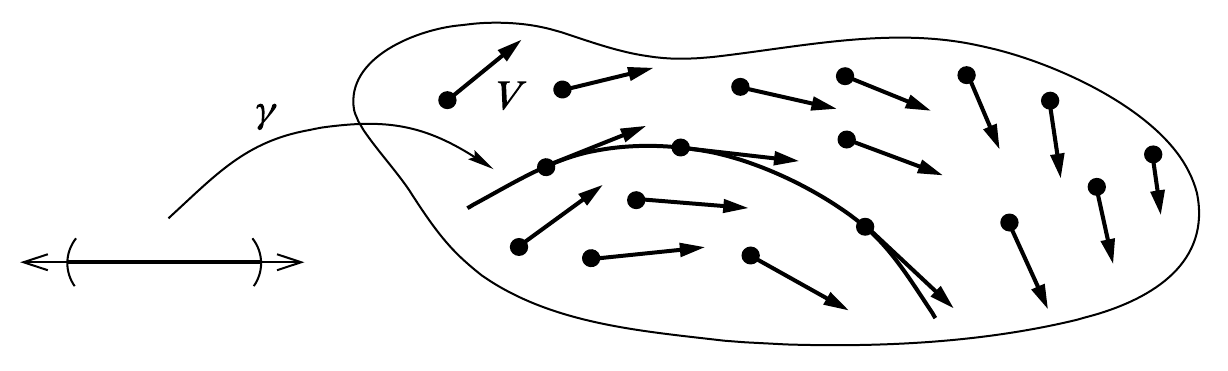
\includegraphics[scale = 0.3]{chapter09/c9f1.png}
\end{center}

\setcounter{thm}{1}

\begin{prop}
Let $V$ be a smooth vector field on a smooth manifold $M$. For each point $p\in M$, there exists $\vep > 0$ and a smooth curve $\ga(-\vep, \vep)\ra M$ that is an integral curve of $V$ starting at $p$.
\end{prop}


\begin{lem}[Rescaling Lemma]
Let $V$ be a smooth vector field on a smooth manifold $M$, let $J\seq \R$ be an interval, and let $\ga:J\ra M$ be an integral curve of $V$. For any $a\in \R$, the curve $\td\ga:\td J\ra M$ defined by $\td\ga(t) = \ga(at)$ is an integral curve of the vector field $aV$, where $\td J = \{t\ :\ at \in J\}$.
\end{lem}

\begin{lem}[\hlb{Translation Lemma}]
Let $V, M, J$ and $\ga$ be as in the preceding lemma. For any $b\in \R$, the curve $\wh\ga:\wh J\ra M$ defined by $\wh\ga(t) = \ga(t + b)$ is also an integral curve of $V$, where $\wh J = \{t\ :\ t + b \in J\}$.
\end{lem}

\begin{prop}[Naturality of Integral Curves]
Suppose $M$ and $N$ are smooth manifold and $F:M\ra N$ is a smooth map. Then $X\in \fkX(M)$ and $Y\in \fkX(N)$ are $F$-related if and only if $F$ tales integral curve so of $X$ to integral curves of $Y$, meaning that for each integral curve of $X$, $F\circ \ga$ is an integral curve of $Y$.
\end{prop}

\dfn We define a \df{global flow} on $M$ (also called a \df{one-parameter group action}) to be a continuous left $\R$-action on $M$; that is, a continuous map $\theta:\R\x M\ra M$ satisfying the following properties for all $s,t\in \R$ and $p\in M$:
\[\theta(t,\theta(s,p)) = \theta(t + x, p),\qquad \theta(0,p) = p.\]

\dfn Given a global flow $\theta$ on $M$, we define two collections of maps as follows:
\begin{itemize}
    \item For each $t\in \R$, define a continuous map $\theta_t:M\ra M$ by 
    \[\theta_t(p) = \theta(t,p).\]
    \item For each $p\in M$, define a curve $\theta^{(p)}:\R\ra M$ by 
    \[\theta^{(p)}(t) = \theta(t,p).\]
\end{itemize}

\dfn If $\theta:\R\x M\ra M$ is a smooth global flow, for each $p\in M$ we define a tangent vector $V_p\in T_pM$ by 
\[V_p = \theta^{(p)\prime}(0).\]
The assignment $p\mapsto V_p$ is a (rough) vector field om $M$, which is called the \df{infinitesimal generator of $\boldsymbol{\theta}$}.

\setcounter{thm}{6}

\begin{prop}
Let $\theta:\R\x M\ra M$ be a smooth global flow on a smooth manifold $M$. The infinitesimal generator $V$ of $\theta$ is a smooth vector field on $M$, and \hl{each curve $\theta^{(p)}$ is an integral curve of $V$.}
\end{prop}

\begin{center}
    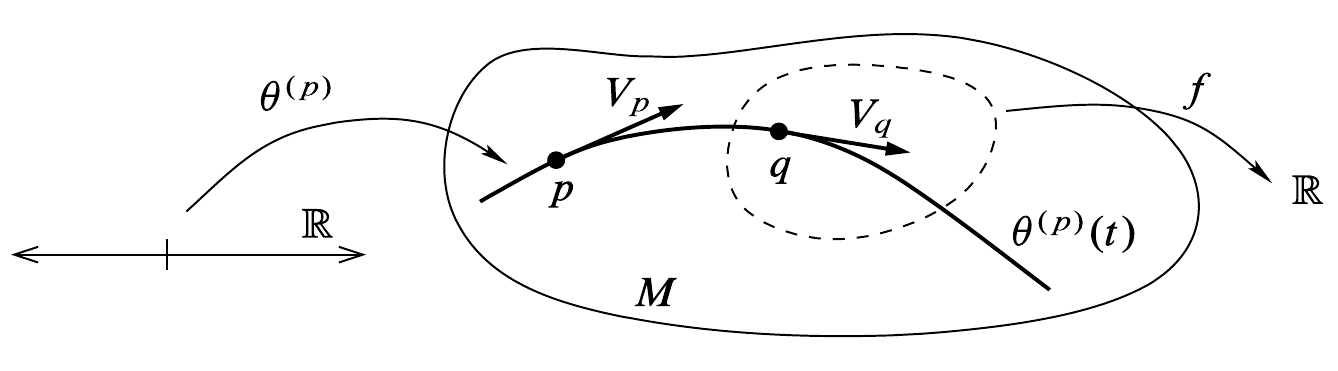
\includegraphics[scale = 0.3]{chapter09/c9f4.png}
\end{center}

\setcounter{thm}{8}

\begin{ex}[Smooth Vector Field that does not Generate a Smooth Global Flow]
Let $M = \R^2\backslash\{0\}$ with standard coordinates $(x,y)$, and let $V$ be the vector field $\pdd{x}$ on $M$. The unique integral curve of $V$ starting at $(-1,0)\in M$ is $\ga(t) = (t - 1, 0)$. However, in this case, $\ga$ cannot be extended continuously past $t = 1$. This is intuitively evident because of the "hole" in $M$ at the origin.
\end{ex}

\dfn If $M$ is a manifold, a \df{flow domain} for $M$ is an open subset $\DD\seq \R\x M$ with the property that for each $p\in M$, the set $D^{(p)} = \{t\in \R\ :\ (t,p)\in \DD\}$ is an open interval containing 0.

\dfn A \df{flow} (or \df{local flow}) on $M$ is a continuous map $\theta:\DD\ra M$, where $\DD\seq \R\x M$ is a flow domain, that satisfies the following group laws: for all $p\in M$
\[\theta(0,p) = p,\]
and for all $s\in \DD^{(p)}$ and $t\in \DD^{(\theta(s,p))}$ such that $s + t \in \DD^{(p)}$,
\[\theta(t,\theta(s,p)) = \theta(t + x, p).\]

\begin{center}
    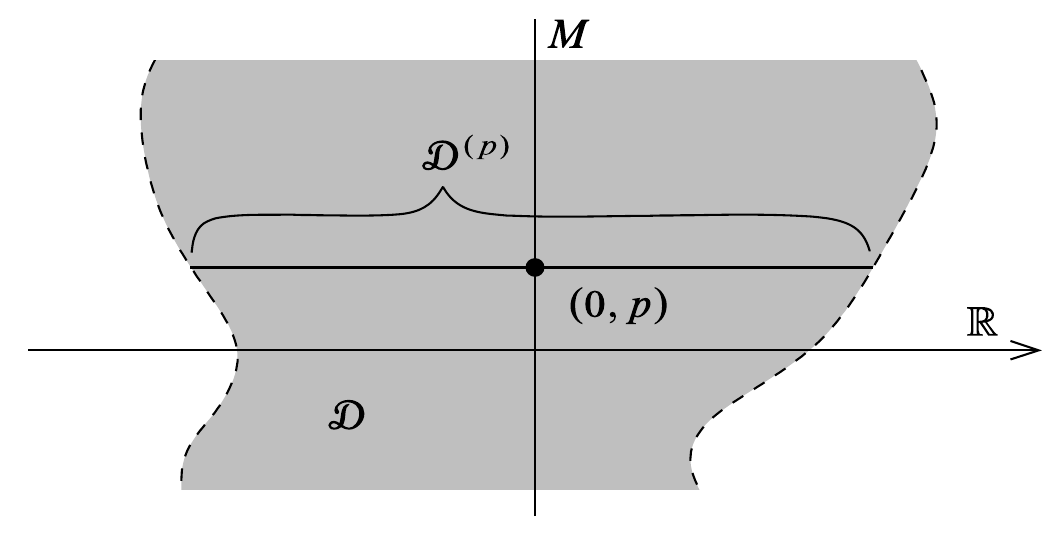
\includegraphics[scale = 0.3]{chapter09/c9f5.png}
\end{center}

\dfn If $\theta$ is a flow, we define $\theta_t(p) = \theta^{(p)} = \theta(t,p)$ whenever $(t,p)\in \DD$. For each $t\in \R$, we also define
\[M_t = \{p\in M\ :\ (t,p)\in \DD\},\]
so that 
\[p\in M_t\Leftrightarrow t\in \DD^{(p)}\Leftrightarrow (t,p)\in \DD.\]
If $\theta$ is smooth, the \df{infinitesimal generator of $\boldsymbol{\theta}$} is defined by $V_p = \theta^{(p)\prime}(0)$.

\setcounter{thm}{10}

\begin{prop}
If $\theta:\DD\ra M$ is a smooth flow, then the infinitesimal generator $V$ of $\theta$ is a smooth vector field, and each cure $\theta^{(p)}$ is an integral curve of $V$.
\end{prop}

\dfn A \df{maximal integral curve} is one that cannot be extended to an integral curve on any larger open interval, and a \df{maximal flow} is a flow that admits no extension to a flow on a larger flow domain.

\begin{thm}[\hlb{Fundamental Theorem on Flows}]
Let $V$ be a smooth vector field on a smooth manifold $M$. There is a unique smooth maximal flow $\theta:\DD\ra M$ whose infinitesimal generator is $V$. This flow has the following properties:
\begin{enumerate}
    \item For each $p\in M$, the curve $\theta^{(p)}:\DD^{(p)}\ra M$ is the unique maximal integral curve of $V$ starting at $p$.
    \item If $s\in \DD^{(p)}$, then $\DD^{(\theta(s,p))}$ is the interval $\DD^{(p)} - s = \{t - s\ :\ t\in \DD^{(p)}\}$.
    \item For each $t\in \R$, the set $M_t$ is open in $M$, and $\theta_t:M_t\ra M_{-t}$ is a diffeomorphism with inverse $\theta_{-t}$.
\end{enumerate}
\end{thm}

\dfn We say that a smooth vector field is \df{complete} if it generates a global flow, or equivalently if each of its maximal integral curves is defined for all $t\in \R$.

\setcounter{thm}{14}

\begin{lem}[\hlb{Uniform Time Lemma}]
Let $V$ be a smooth vector field on a smooth manifold $M$, and let $\theta$ be its flow. Suppose there is a positive number $\vep$ such that for every $p\in M$, the domain $\theta^{(p)}$ contains $(-\vep,\vep)$. Then $V$ is complete.
\end{lem}

\begin{thm}
Every compactly supported smooth vector field on a smooth manifold is complete.
\end{thm}

\begin{cor}
On a compact smooth manifold, every smooth vector field is complete
\end{cor}

\begin{thm}
\hl{Every left-invariant vector field on a Lie group is complete.}
\end{thm}

\begin{thm}[\hl{Flowout Theorem}]
Suppose $M$ is a smooth manifold, $S\seq M$ is an embedded $k$-dimensional submanifold, and $V\in \fkX(M)$ is a smooth vector field that is nowhere tangent to $S$. Let $\theta\DD\ra M$ be the flow of $V$, let $\OO = (\R\x S)\cap \DD$ and let $\Phi = \theta|_\OO$.
\begin{enumerate}
    \item $\Phi:\OO\ra M$ is an immersion.
    \item $\pdd{t}\in \fkX(\OO)$ is $\Phi$-related to $V$.
    \item There exists a smooth positive function $\de:S\ra \R$ such that the restriction of $\Phi$ to $\OO_\de$ is injective, where $\OO_\de\seq \OO$ is the flow domain 
    \[\OO_\de = \{(t.p)\in \OO\ :\ |t| < \de(p)\}.\]
    Thus, $\Phi(\OO_\de)$ is an immersed submanifold of $M$ containing $S$, and $V$ is tangent to this submanifold.
    \item If $S$ has codimension 1, then $\Phi|_{\OO_\de}$ is a diffeomorphism onto an open submanifold of $M$.
\end{enumerate}
\end{thm}

\dfn The submanifold $\Phi(\OO_\de)\seq M$ in the previous theorem is called a \df{flowout from S along V}.

\dfng If $V$ is a vector field on $M$, a point $p\in M$ is said to be a \df{singular point of V} if $V_p = 0$, and a \df{regular point} otherwise.

\setcounter{thm}{20}

\begin{prop}
Let $V$ be a smooth vector filed on a smooth manifold $M$, and let $\theta:\DD\ra M$ be the flow generated by $V$. If $p\in M$ is a singular point of $V$, then $\DD\op = \R$ and $\theta\op$ is the constant curve $\theta\op(t)\equiv p$. If $p$ is a regular point, then $\theta\op:\DD\op\ra M$ is a smooth immersion.
\end{prop}

\begin{thm}[\hlb{Canonical Form Near a Regular Point}]
Let $V$ be a smooth vector field on a smooth manifold $M$, and let $p\in M$ be a regular point of $V$. There exist smooth coordinates $(s^i)$ on some neighborhood of $p$ in which $B$ has the coordinate representation $\pdd{s^1}$. If $S\seq M$ is any embedded hypersurface (submanifold with codimension 1) with $p\in S$ and $V_P\nin T_pS$, then the coordinates can also be chosen so that $s^1$ is a local defining function for $S$.
\end{thm}


\begin{ex}
Let $W = x\pdd{y} - y\pdd{x}$ on $\R^2$. The flow of $W$ is given by 
\[\theta_t(x,y) = (x\cos(t) - y\sin(t), x\sin(t) + y\cos(t).\]
The point $(1,0)\in \R^2$ is a regular point of $W$ because $W_{(1,0)} = \ev{\pdd{y}}{(1,0)}\neq 0$. Because $W$ has nonzero $y$-coordinate there, we can take $S$ to be the $x$-axis, parameterized by $X(s) = (s,0)$. We define $\Psi:\R^2\ra R^2$ by 
\[\Psi(t,s) = \theta_t(s,0) = (s\cos(t), s\sin(t)),\]
and then solve locally for $(t,s)$ in terms of $(x,y)$ to obtain the following coordinate map in a neighborhood of $(1,0)$:
\[(t,s) = \Psi\inv(x,y) =\lp \tan\inv\lp\frac{y}{x}\rp,\sqrt{x^2 + y^2}\rp.\]
It is easy to check that $W = \pdd{t}$ in these coordinates.
\end{ex}



\subsection{Lie Derivatives}\nl

\dfn Let $M$ be a smooth manifold, $V$ a smooth vector field on $M$, and $\theta$ the flow of $V$. For any smooth vector field $W$ on $M$, define a rough vector field on $M$, denoted by $\LL_V W$ and called the \df{Lie derivative of W with respect to V}, by 
\begin{align*}
    (\LL_V W)_p &= \ev{\frac{d}{dt}}{t = 0}d(\theta_{-t})_{\theta_t(p)}(W_{\theta_t(p)})\\
    &=\lim_{t\ra 0} \frac{d(\theta_{-t})_{\theta_t(p)}(W_{\theta_t(p)}) - W_p}{t},
\end{align*}
provided the derivative exists.

\begin{center}
    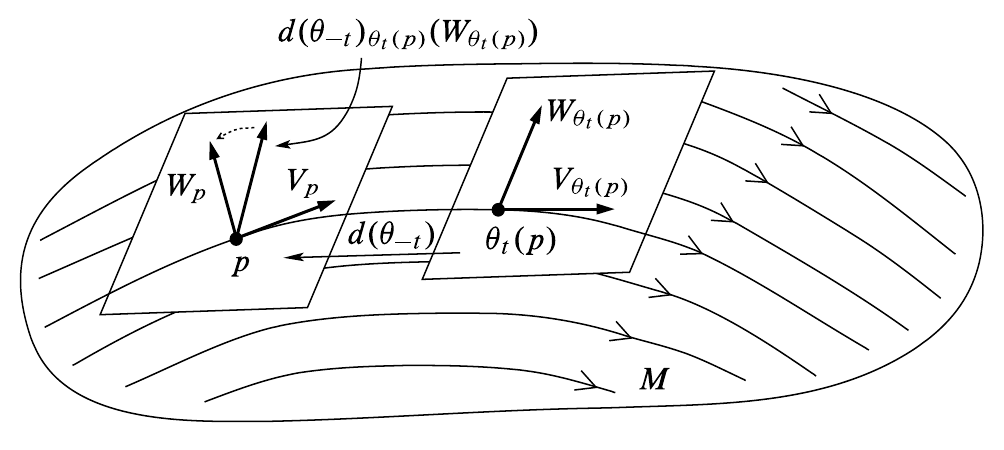
\includegraphics[scale = 0.38]{chapter09/c9f13.png}
\end{center}

\setcounter{thm}{35}

\begin{lem}
Suppose $M$ is a smooth manifold \wowob, and $V,W\in \fkX(M)$. If $\bd M\neq \es$, assume in addition that $V$ is tangent to $\bd M$. Then $(\LL_pW)_p$ exists for every $p\in M$, and $\LL_V W$ is a smooth vector field.
\end{lem}

\setcounter{thm}{37}

\begin{thm}
\hlb{If $M$ is a smooth manifold and $V,W\in \fkX(M)$ then $\LL_V W = [V,W]$.}
\end{thm}


\begin{cor}
Suppose $M$ is a smooth manifold \wowob, and $V,W,X\in \fkX(M)$.
\begin{enumerate}
    \item $\LL_V W = - \LL_W V$.
    \item $\LL_V [W,X] = [\LL_VW,X] + [W,\LL_VX]$.
    \item $\LL_{[V,W]}X = \LL_V\LL_W X - \LL_W\LL_V X$.
    \item If $g\in \Cin(M)$, then $\LL_V(gW) = (Vg)W + g\LL_VW$.
    \item If $F:M\ra N$ is a diffeomorphism, then $F_*(\LL_VX) = \LL_{F_*V}F_*X$.
\end{enumerate}
\end{cor}

\setcounter{thm}{40}

\begin{prop}
Suppose $M$ is a smooth manifold \wowob and $<W\in \fkX(M)$. If $\bd M \neq \es$, assume also that $V$ is tangent to $\bd M$. Let $\theta$ be the flow of $V$. For any $(t_0, p)$ in the domain of $\theta$,
\[\ev{\frac{d}{dt}}{t = t_0}d(\theta_{-t})_{\theta_t(p)}(W_{\theta_t(p)}) = d(\theta_{-t_0})\big((\LL_V W)_{\theta_{t_0}(p)}\big)\]
\end{prop}

\dfng Let $M$ be a smooth manifold and $V,W\in \fkX(M)$. We say that \df{V and W commute} if $VWf = WVf$ for every smooth function $f$, or equivalently if $[V,W] \equiv 0$.

\dfn If $\theta$ is a smooth flow, a vector field $W$ is said to be \df{invariant under $\boldsymbol{\theta}$} it $W$ is $\theta_t$-related to itself for each $t$, i.e., if
\[(d\theta_t)_p(W_p) = W_{\theta_t(p)}\]
for all $(t,p)$ in the domain of $\theta$.

\begin{thm}
For smooth vector fields $V$ and $W$ on a smooth manifold $M$, the following are equivalent:
\begin{enumerate}
    \item $V$ and $W$ commute.
    \item $W$ is invariant under the flow of $V$.
    \item $V$ is invariant under the flow of $W$.
\end{enumerate}
\end{thm}

\begin{cor}
Every smooth vector field is invariant under its own flow.
\end{cor}

\dfn if $\theta, \psi$ are flows on $M$, we say that \df{$\boldsymbol{\theta}$ and $\boldsymbol{\psi}$ commute} if for all $p\in M$ whenever $J,K\seq \R$ are open intervals containing 0 such that one of the expression $\theta_t\circ\psi_s(p)$ or $\psi_s\circ \theta_t(p)$ is defined for all $(s,t)\in J\x K$, both are defined and they are equal.

\begin{thm}
Smooth vector fields commute if and only if their flows commute.
\end{thm}

\dfn Suppose $M$ is a smooth $n$-manifold. A smooth local frame $(E_i)$ for $M$ is called a \df{commuting frame} if $[E_i,E_j] = 0$ for all $i$ and $j$.

\setcounter{thm}{45}

\begin{thm}[\hlb{Canonical Form for Commuting Vector Fields}]
Let $M$ be a smooth $n$-manifold, and let $(V_1,\ldots,V_k)$ be a linearly independent $k$-tuple of smooth commuting vector fields on an open subset $W\seq M$. For each $p\in W$, there exists a smooth coordinate chart $(U, (s^i))$ centered at $p$ such that $V_i = \pdd{s^i}$ for $i = 1,\ldots,k$. If $S\seq W$ is an embedded codimension-$k$ submanifold and $p$ is a point of $S$ such that $T_pS$ is complementary to the span of $V_1|_p,\ldots,V_k|_p)$, then the coordinates can also be chosen such that $S\cap U$ is the slice define by $s^1 = \cdots = s^k = 0$.
\end{thm}

\begin{ex}
Consider the following two vector fields on $\R^2$:
\[V = x\pdd{y}-y\pdd{x},\qquad W = x\pdd{x} + y\pdd{y}.\]
A computation shows that $[V,W] = 0$. And Example 9.23 showed us that the flow of $V$ is given by 
\[\theta_t(x,y) = (x\cos(t) - y\sin(t), x\sin(t) + y\cos(t),\]
and an easy verification show that the flow of $W$ is 
\[\eta_t(x,y) = (e^t x, e^t y).\]
At $p = (1,0)$, $V_p$ and $W+p$ are linearly independent. Because $k = n = 2$ in this case, we can take the subset $S$ to be the single point $\{(1,0)\}$, and define $\Phi:\R^2\ra \R^2$ by 
\[\Phi(s,t) = \eta_t\circ \theta_s(1,0) = (e^t\cos(s),e^t\sin(s)).\]
In this case, we can solve for $(s,t) = \Phi\inv(x,y)$ explicitly in a neighborhood of $(1,0)$ to obtain the coordinate map 
\[(s,t) = \lp\tan\inv\lp\frac{y}{x}\rp,\log\lp\sqrt{x^2 + y^2}\rp\rp.\]
\end{ex}

























\newpage
\setcounter{section}{11}
\section{The Seifert-van Kampen Theorem}
\vs


\dfn Push-out diagrams and amalgamated products. Let $A_1,\ A_2,\ B$ be groups with
\begin{center}
    \begin{tikzcd}
        B\arrow[r, "f_1"]\arrow[d, "f_2", swap] & A_1\arrow[d, "g_1"]\arrow[ddr, bend left, "h_1"]&\\
        A_2\arrow[r, swap, "g_2"]\arrow[drr, bend right, swap, "h_2"] & C\arrow[dr, dashed, "\exists ! \vphi"] & \\
        & & D
    \end{tikzcd}
\end{center}
where $(C, g_1, g_2)$ is a unique solution that satisfies the universal property.

\textbf{Note:} If $B$ is trivial, then $C$ is the free product $A_1*A_2$ of $A_1$ and $A_2$, i.e. $C$ is the free group generated by $A_1$ and $A_2$.

\textbf{Seifert-van Kampen Theorem} (Baby Case) Assume that $X = A\cup B$ with $A\cap B$ path-connected, locally path-connected, and $\pi_1(A\cap B) = 1$. Then we have that $\pi_1(X, x_0) \cong \pi(A, x_0) * \pi(B, x_0)$.

\dfn Will denote the join of two spaces $X\vee Y$ where the join glues together the two spaces at exactly one point.

\textbf{Seifert-van Kampen Theorem} (General Case) Let $X = U\cup V$, where $U$ and $V$ are open in $X$; assume $U, V,$ and $U\cap V$ are path connected; let $x_0\in U\cap V$. Let $H$ be a group, and let
\[\vphi_1:\pi_1(U, x_0)\ra H\qquad\text{and}\qquad\vphi_2:\pi_1(V,x_0)\ra H\]
be homomorphisms. Let $i_1,i_2,j_1,j_2$ be the homomorphisms indicated in the following diagram, each induced by inclusion.
\begin{center}
\begin{tikzcd}
 & \pi_1(U,x_0)\arrow[dr, "\vphi_1"]\arrow[d, "j_1"] & \\
 \pi_1(U\cap V, x_0)\arrow[ur, "i_1"]\arrow[r]\arrow[dr, swap, "i_2"] & \pi_1(X, x_0)\arrow[dotted, r, "\Phi"] & H \\
 & \pi_1(V, x_0)\arrow[u, swap, "j_2"]\arrow[ur, swap, "\vphi_2"] &
\end{tikzcd}
\end{center}
If $\vphi_1\circ i_1 = \vphi_2\circ i_2$, then there is a unique homomorphism $\Phi:\pi_1(X, x_0)\ra H$ such that $\Phi\circ j_1 = \vphi_1$ and $\Phi\circ j_2 = \vphi_2$.





% %==========================================================================
% %                    SECTION 51
% %==========================================================================
% \subsection{Homotopy of Paths}\nl
% \setcounter{section}{51}
% \setcounter{thm}{0}

\newpage\setcounter{section}{13}
\section{Differential Forms}

Differential forms are an essential and beautiful part of Differential Geometry. They are, in fact, the objects that we will use in order to thoroughly define the concept of integration on an arbitrary smooth manifold. And, as we will find in Chapter 16, their very existence is what leads to a very elegant and concise way of expressing Stokes's Theorem.

\dfn Let $V, W$ be finite dimensional vector fields, and let $\al\in V^*$ and $\be \in W^*$. The \df{tensor product} $\al\otimes\be$ is a bilinear product
\[\al\otimes\be:V\x W\ra \R:(v,w)\mapsto \al(v)\be(w).\]

\nb To define $v\otimes w$ for $v\in V$ and $w\in W$, use the canonical identification with the double dual.

\dfn Let $\al,\be\in V^*$. The \df{wedge product} of $\al$ and $\be$ is defined by
\[\al\wedge\be = \al\otimes \be - \be\otimes \al.\]

\dfn The space of \df{alternating k-vectors} or \df{alternating k-covectors} of $V^*$ is
\[\bgw^kV^* = \spn\{\al^1\wedge\cdots\wedge\al^k\ :\ \al^i\in V^*\}\]

\nb For $0\leq k \leq n = \dim(V)$, $\dim(\bgw^kV^*) = {n \choose k}$

\setcounter{thm}{10}

\begin{prop}[Properties of the Wedge Product] Suppose $\omega,\omega\p,\eta,\eta\p$, and $\xi$ are multicovectors on a finite-dimensional vector space $V$.
\begin{enumerate}
    \item {\scshape Binlearity:} For $a,a\p\in \R$,
    \begin{align*}
        [(a\omega + a\p\omega\p)\wedge\eta = a(\omega\wedge\eta) + a\p(\omega\p\wedge\eta),\\
        \eta\wedge(a\omega + a\p\omega\p) = a(\eta\wedge\omega) + a\p(\eta\wedge\omega\p).
    \end{align*}
    \item {\scshape Associativity:}
        \[\omega\wedge(\eta\wedge\xi) = (\omega\wedge\eta)\wedge\xi.\]
    \item {\scshape Anticommutativity:} For $\omega\in\bgw^k(V^*)$ and $\eta\in\bgw^\ell(V^*)$
    \[\omega\wedge\eta = (-1)^{k\ell}\eta\wedge\omega.\]
    \item If $(\vep^i)$ is any basis for $V^*$ and $I = (i_1,\ldots,i_k)$ is any multi-index, then
    \[\vep^{i_1}\wedge\vep^{i_k} = \vep^I.\]
    \item \hl{For any covectors $\omega^1,\ldots,\omega^k$ and vectors $v_1,\ldots,v_k$,}
    \[\omega^1\wedge\cdots\wedge\omega^k(v_1,\ldots,v_k) = \det(\omega^j(v_i)).\]
\end{enumerate}
\end{prop}


\dfn A $k$-covector $\eta$ is \df{decomposable} if it can be expressed as
\[\eta = \omega^1\wedge \cdots\wedge \omega^k\]
where $\omega^i$ is a covector.

\dfn for any $n$-dimensional vector space $V$, the \df{exterior algebra} of $V$ is the vector space
\[\bgw(V^*) = \bigotimes_{k = 0}^n \bgw^k V\]


\dfn Let $V$ be a finite-dimensional vector space. For each $v\in V$, we define a linear map $i_v:\bgw^k(V^*)\ra\bgw^{k - 1}(V^*)$, called \df{interior multiplication by v}, as follows:
\[i_v\omega(w_1,\ldots,w_{k - 1}) = \omega(v,w_1,\ldots,w_{k - 1}).\]
In other words, $i_v\omega$ is obtained from $\omega$ by inserting $v$ into the first slot. This can also be denoted by $v\hook \omega$.

\setcounter{thm}{12}

\begin{lem}
Let $V$ be a finite-dimensional vector space and $v\in V$.
\begin{enumerate}
    \item $i_v\circ i_v = 0$.
    \item If $\omega\in \bgw^k(V^*)$ and $\eta\in \bgw^\ell(V^*)$,
    \[i_v(\omega\wedge\eta) = (i_v\omega)\wedge\eta + (-1)^k\omega\wedge(i_v\eta)\]
\end{enumerate}
\end{lem}

\dfn The \df{bundle of alternating k-tensors} on a smooth manifold $M$ is
\[\Lambda^k(T^*M) = \bigsqcup_{p\in M} \Lambda(T^*_pM).\]


\dfn A \df{differential k-form} on $M$ is a continuous section of $\Lambda^k(T^*M)$. The vector space of smooth $k$-forms is denoted
\[\Omega^k(M) = \Gamma(\Lambda(T^*M)),\]
and the integer $k$ is called the \df{degree} of the form.

\dfn WE define the vector space $\Omega^*(M)$ to be
\[\Omega^*(M) = \bigoplus_{k = 0}^n \Omega^k(M),\]
and this is an associative, anticommutative graded algebra.


\setcounter{thm}{15}

\begin{lem}
Suppose $F:M\ra N$ is smooth.
\begin{enumerate}
    \item $F^*:\Omega^k(N)\ra \Omega^k(M)$ is linear over $R$.
    \item $F^*(\omega\wedge\eta) = (F^*\omega)\wedge(F^*\eta)$.
    \item In any smooth chart
    \[F^*\lp{\sum_I}\p\omega_I\,dy^{i_1}\wedge\cdots\wedge dy^{i_k}\rp = {\sum_I}\p(\omega_I\circ F)\,d(y^{i_1}\circ F)\wedge\cdots\wedge d(y^{i_k}\circ F)\]
\end{enumerate}
\end{lem}

\setcounter{thm}{19}

\begin{prop}[\hlb{Pullback Formula for Top-Degree Forms}]
Let $F:M\ra N$ be a smooth map between $n$-manifolds \wowob. If $(x^i)$ and $(y^j)$ are smooth coordinates on open subsets $U\seq M$ and $V\seq N$, respectively, and $u$ is a continuous real-valued function on $V$, then the following holds on $U\cap F\inv(V)$:
\[F^*(u\,dy^1\wedge\cdots\wedge dy^n) =(u\circ F)(\det(DF))\,dx^1\wedge\cdots\wedge dx^n,\]
where $DF$ represents the Jacobian matrix of $F$ in these coordinates.
\end{prop}

\dfn Let $\omega = \sum_{|I| = k} f_I\, dx^{i_1}\wedge\cdots\wedge dx^{i_k}$ be a $k$-form on $\Rn$. The \df{exterior derivative} of $\omega$ is the $(k + 1)$-form
\[d\omega = \sum_{|I| = k} df_I\wedge dx^{i_1}\wedge\cdots\wedge dx^{i_k}.\]

\setcounter{thm}{22}

\begin{prop}[\hl{Properties of the Exterior Derivative on $\boldsymbol{\Rn}$}]\nl
\begin{enumerate}
    \item $d$ is linear over $\R$.
    \item If $\omega$ is a smooth $k$-form and $\eta$ is a smooth 1-form on an open subset $U\seq \Rn$ or $\Hn$, then
    \[d(\omega\wedge\eta) = d\omega\wedge\eta + (-1)^k\omega\wedge d\eta.\]
    \item \hlb{$d\circ d\equiv 0$}
    \item $d$ commutes with pullbacks.
\end{enumerate}
\end{prop}

\begin{thm}[Existence and Uniqueness of Exterior Differentiation]
Suppose $M$ is a smooth manifold \wowob. There are unique operators $d:\Omega^k(M)\ra \Omega^{k + 1}(M)$ for all $k$, called \df{exterior differentiation}, satisfying the following four properties:
\begin{enumerate}[(i)]
    \item $d$ is linear over $\R$.
    \item If $\omega\in\Omega^k(M)$ and $\eta \in \Omega^\ell(M)$, then
    \[d(\omega\wedge\eta) = d\omega\wedge\eta + (-1)^k\omega\wedge\eta.\]
    \item $d\circ d \equiv 0$.
    \item for $f\in \Omega^0(M) = \Cin(M)$, $df$ is the differential of $f$, given by $df(X) = Xf$.
\end{enumerate}
\end{thm}

\setcounter{thm}{25}

\begin{prop}[Naturality of the Exterior Derivative]
If $F:M\ra N$ is a smooth map, then for each $k$ the pullback map $F^*:\Omega^k(N)\ra \Omega^k(M)$ commutes with $d$: for all $\omega\in \Omega^k(N)$,
\[F^*(d\omega) = d(F^*\omega).\]
\end{prop}

Now, the particularly astute will notice that the exterior derivative seems to act very similarly to the vector field operations that we encountered in Calculus III. This is no happy accident! In fact, when we define the three operations
\begin{align*}
    \flat &:\fkX(\R^3)\ra \Omega^1(\R^3): X^ie^i \mapsto X_ie^i\\
    \be &: \fkX(\R^3)\ra \Omega^1(\R^3): X \mapsto X\hook (dx\wedge dy\wedge dz)\\
    * &: \Cin(\R^3)\ra \Omega^3(\R^3): f \mapsto f\, dx\wedge dy\wedge dz,
\end{align*}
then we can construct the following pretty commutative diagram:
\begin{center}
\begin{tikzcd}[column sep = 1.5em]
    \Cin(\R^3)\arrow[r, "\text{grad}"]\arrow[d, "\Id"]    &    \fkX(\R^3)\arrow[r, "\text{div}"]\arrow[d, "\flat"]   &    \fkX(\R^3)\arrow[r, "\text{curl}"]\arrow[d, "\be"]   &   \Cin(\R^3)\arrow[d, "*"]\\
    \Omega^0(\R^3)\arrow[r, "\text{d}", swap]   &   \Omega^1(\R^3)\arrow[r, "\text{d}", swap]   &   \Omega^2(\R^3)\arrow[r, "\text{d}", swap]   &    \Omega^3(\R^3)
\end{tikzcd}
\end{center}
This is really nice to keep in mind whenever you are teaching Calc. III.

\setcounter{thm}{28}

\begin{prop}[Exterior Derivative of a 1-Form]
For any smooth 1-form $\omega$ and smooth vector fields $X$ and $Y$,
\[d\omega(X,Y) = (X(\omega(Y)) - Y(\omega(X)) - \omega([X,Y]).\]
\end{prop}

\begin{prop}
Let $M$ be a smooth $n$-manifold \wowob, let $(E_i)$ be a smooth local frame for $M$, and let $(\vep^i)$ be the dual coframe. For each $i$, let $b^i_{jk}$ denote the component functions of the exterior derivative of $\vep^i$ in this frame , and for each $j,k$, let $c^i_{jk}$ be the component functions of the Lie bracket $[E_j,E_k]$:
\[d\vep^i = \sum_{j < k}b^i_{jk}\vep^j\wedge\vep^k;\qquad [E_j,E_k] = c^i_{jk}E_i.\]
Then $b^i_{jk} = -c^i_{jk}$.
\end{prop}

\dfng A $k$-form on $\Rn$ is called \df{closed} if $d\omega = 0$ and \df{exact} if $\omega = d\eta$ for some $(k - 1)$-form $\eta$ on $\Rn$.

\setcounter{thm}{32}

\begin{prop}
Suppose $M$ is a smooth manifold $V\in \fkX(M)$, and $\omega\eta\in\Omega^*(M)$. Then
\[\LL_V(\omega\wedge\eta) = \LL_V\omega\wedge\eta + \omega\wedge(\LL_V\eta).\]
\end{prop}

\setcounter{thm}{34}

\begin{thm}[\hl{Cartan's Magic Formula}]
On a smooth manifold $M$, for any smooth vector field $V$ and any smooth differential form $\omega$,
\[\LL_V\omega = V\hook (d\omega) + d(V\hook \omega).\]
\end{thm}

\begin{cor}
If $V$ is a smooth vector filed and $\omega$ is a smooth differential form, then
\[\LL_V(d\omega) = d(\LL_V\omega).\]
\end{cor}

\newpage\setcounter{section}{14}
\section{Orientations}

This section is mainly here to provide structure and terminology for what is to come in Chapter 16.

\dfn Let $V$  be a real vector space of dimension $n\geq 1$. We say that two ordered bases $(E_i)$ and $\td E_j)$ for $V$ are \df{consistently oriented} if the transition matrix $(B^j_i)$, defined by 
\[E_i = B^j_i \td E_j,\]
has positive determinant.

\nb The motivation for this definition is that we want things with the same orientation to not flip the sign on the volume form.

\dfn If $\dim(V) = N\geq 1$, we define an \df{orientation for V} as an equivalence class of ordered bases. If $(E_1,\ldots,E_n)$ is any ordered basis for $V$, we denote the orientation that it determines by $[E_1,\ldots,E_n]$. A vector space together with a choice of orientation is called an \df{oriented vector space}. If $V$ is oriented, then any ordered basis $(E_1,\ldots,E_n)$ that is in the given orientation is said to be \df{positively oriented}.

\dfn Let $M$ be a smooth manifold \wowob. We define a \df{pointwise orientation} on $M$ to be a choice of orientation of each tangent space.

\dfn Let $M$ be a smooth $n$-manifold \wowob, endowed with a pointwise orientation. If $(E_i)$ is a local frame for $TM$, we say that $(E_i)$ is \df{(positively) oriented} if $(\ev{E_1}{p},\ldots\ev{E_n}{p})$ is a positively oriented basis for $T_pM$ at each point.

\setcounter{thm}{4}

\begin{prop}[\hl{The Orientation Determined by an $\boldsymbol{n}$-form}]
Let $M$ be a smooth $n$-manifold \wowob. Any nonvanishing $N$-form $\omega$ on $M$ determines a unique orientation of $M$ for which $\omega$ is positively oriented at each point. Conversely, if $M$ is given an orientation, then there is a smooth nonvanishing $n$-form on $M$ that is positively oriented at each point.
\end{prop}


\dfn Any nonvanishing $n$-form on $M$ is called an \df{orientation form}.

\dfn A smooth coordinate chart on an oriented smooth manifold \wowob is said to be \df{(positively) oriented} if the coordinate frame $\lp\pdd{x^i}\rp$ is positively oriented. A smooth atlas $\{(U_\al, \vphi_\al)\}$ is said to be \df{consistently oriented} if for each $\al,\be$ the transition map $\vphi_\be\circ\vphi_\al\inv$ has positive Jacobian determinant everywhere on $\vphi_\al(U_\al\cap U_\be)$.

\begin{prop}[The Orientation Determined by a Coordinate Atlas]
Let $M$ be a smooth positive-dimensional manifold \wowob. Given any consistently oriented smooth atlas for $M$, there is a unique orientation for $M$ with the property that each chart in the given atlas is positively oriented. Conversely, if $M$ is oriented and either $\bd M = \es$ or $\dim(M) > 1$, then the collection of all oriented smooth charts is a consistently oriented atlas for $M$.
\end{prop}

\dfng Let $M$ and $N$ be oriented smooth manifold \wowob, and suppose $F:M\ra N$ is a local diffeomorphism. If $M$ and $N$ are positive-dimensional, we say that $F$ is \df{orientation-preserving} if for each $p\in M$, the isomorphism $dF_p$ takes oriented basis of $T_pM$ to oriented basis of $T_{F(p)}N$.

\setcounter{thm}{14}

\begin{prop}[The Pullback Orientation]
Suppose $M$ and $N$ are smooth manifolds \wowob. If $F:M\ra N$ is a local diffeomorphism and $N$ is oriented, then $M$ has a unique orientation, called the \df{pullback orientation induced by F}, such that $F$ is orientation-preserving.
\end{prop}

\setcounter{thm}{16}

\begin{prop}
\hlb{Every parallelizable smooth manifold is orientable.}
\end{prop}

\setcounter{thm}{20}

\begin{prop}
Suppose $M$ is an oriented smooth $n$-manifold \wowob, $S$ is an immersed hypersurface \wowob in $M$, and $N$ is a vector field along $S$ that is nowhere tangent to $S$. Then $S$ has a unique orientation such that for each $p\in S$, $(E_1,\ldots,ER_{n - 1})$ is an oriented basis for $T_pS$ if and only if $(N_p,E_1,\ldots,E_{n - 1})$ is an oriented basis for $T_pM$. If $\omega$ is an orientation form for $M$, then $\iota^*_S(N\hook \omega)$ is an orientation form for $S$ with respect to this orientation, where $\iota_S:S\into M$ is inclusion.
\end{prop}

\setcounter{thm}{23}

\begin{prop}[\hlb{The Induced Orientation on a Boundary}]
Let $M$ be an oriented smooth $n$-manifold with boundary, $n\geq 1$. Then $\bd M$ is orientable, and all outward-pointing vector fields along $\bd M$ determine the same orientation on $\bd M$.
\end{prop}

\newpage\setcounter{section}{15}
\section{Integration on Manifolds}

Really all we want to talk about here is Stokes's Theorem.

\begin{prop}
Suppose $D$ and $E$ are open domains of integration in $\Rn$ or $\Hn$, and $G:\ol D \ra \ol E$ is a smooth map that restricts to an orientation-preserving or orientation-reversing diffeomorphism from $D$ to $E$. If $\omega$ is an $n$-form on $\ol E$, then 
\[\int_D G^*\omega = \begin{cases} \int_E \omega & \text{if $G$ is orientation-preserving},\\
-\int_E \omega & \text{if $G$ is orientation-reversing}.\end{cases}\]
\end{prop}

\begin{lem}
Suppose $U$ is an open subset of $\Rn$ or $\Hn$, and $K$ is a compact subset of $U$. Then there is an open domain of integration $D$ such that $K\seq D\seq \ol D\seq U$.
\end{lem}

\begin{prop}
Suppose $U, V$ are open subsets of $\Rn$ or $\Hn$, and $G:U\ra V$ is an orientation preserving or orientation reversing diffeomorphism. If $\omega$ is a compactly supported $n$-form on $V$, then
\[\int_V\omega = \pm\int_U G^*\omega,\]
with the positive sing if $G$ is orientation-preserving, and the negative sign otherwise.
\end{prop}

\dfn Suppose that $\omega$ is an $n$-form on $M$ that is compactly supported in the domain of a single smooth chart $(U,\vphi)$ that is either positively or negatively oriented. We define the \df{integral of $\boldsymbol{\omega}$ over M} to be
\[\int_M\omega = \pm\int_{\vphi(U)}(\vphi\inv)^*\omega.\]

\begin{prop}
With $\omega$ as above, $\int_M\omega$ does not depend on the choice of smooth chart whose domain contains $\supp(\omega)$.
\end{prop}

\begin{prop}
The definition of $\int_M\omega$ above does not depend on the choice of chart or partition of unity.
\end{prop}

\begin{prop}[\hl{Properties of Integrals of Forms}]
Suppose $M$ and $N$ are non-empty oriented smooth $n$-manifolds \wowob, and $\omega, \eta$ are compactly supported $n$-forms on $M$.
\begin{enumerate}
    \item {\scshape Linearity:} If $a,b\in \R$, then
    \[\int_M a\omega + b\eta = a\int_m\omega + b\int_M \eta.\]
    \item {\scshape Orientation Reversal:} If $-M$ denotes $M$ with the opposite orientation, then
    \[\int_{-M}\omega = -\int_M\omega.\]
    \item {\scshape Positivity:} If $\omega$ is a positively oriented orientation form, then $\int_M\omega > 0$.
    \item {\scshape Diffeomorphism Invariance:} If $F:N\ra M$ is an orientation-preserving or orientation reversing diffeomorphism
    \[\int_M\omega = \begin{cases} \int_N F^*\omega & \text{if $F$ is orientation-preserving,}\\ -\int_N F^*\omega & \text{if $F$ is orientation-reversing.}\end{cases}\]
\end{enumerate}
\end{prop}


\setcounter{thm}{10}

\begin{thm}[\hlb{Stokes's Theorem}]
Let $M$ be an oriented smooth $n$-manifold with boundary, and let $\omega$ be a compactly supported smooth $(n - 1)$-form on $M$. Then
\[\int_m d\omega = \int_{\bd M}\omega.\]
\end{thm}

\setcounter{thm}{12}

\begin{cor}[Integrals of Exact Forms]
If $M$ is a compact oriented smooth manifold without boundary, then the integral of every exact form over $M$ is zero:
\[\int_M d\omega = 0 \quad \text{if $\bd M = 0$}.\]
\end{cor}

\begin{cor}[Integrals of Closed Forms over Boundaries]
Suppose $M$ is a compact oriented smooth manifold with boundary. If $\omega$ is a closed form on $M$, then the integral of $\omega$ over $\bd M$ is zero:
\[\int_{\bd M} \omega = 0\quad\text{if $d\omega = 0$ on $M$}.\]
\end{cor}

\begin{cor}
Suppose $M$ is a smooth manifold \wowob, $S\seq M$ is an oriented compact smooth $k$-dimensional submanifold (without boundary), and $\omega$ is a closed $k$-form on $M$. If $\int_S\omega \neq 0$, then both of the following are true:
\begin{enumerate}[(i)]
    \item $\omega$ is not exact on $M$.
    \item $S$ is not the boundary of an oriented compact smooth submanifold with boundary in $M$.
\end{enumerate}
\end{cor}



\end{document}
